\chapter{Data Analysis And Systematic Uncertainties}
\label{ch:analysis}

This chapter describes the statistical and mathematical framework used to analyze the data collected during the 2024 antihydrogen ground-state hyperfine splitting campaign. The improvements in trapping efficiency, magnetic field design, colder energy distribution and characterization of the magnetic field drift, together with new analysis techniques, have all contributed to an improvement of \num{e2} compared to the first observation made by the ALPHA collaboration in 2017 \cite{ALPHA:2017fsh}.

The 2024 dataset consists of two complete spectroscopy campaigns performed at different magnetic-field configurations, together with dedicated auxiliary measurements, including electron cyclotron resonance (ECR) magnetometry and high-statistics calibration samples. These auxiliary datasets play a crucial role in the characterization of the magnetic-field evolution and in the evaluation of systematic uncertainties.

The analysis follows a frequentist approach and is implemented within the \textit{ROOT} and \textit{RooFit} frameworks using a Python-based \textit{PyROOT} analysis package. The model parameters are determined through a maximum-likelihood fit, with numerical minimization performed using the \textit{MINUIT2} optimizer.

The first stage of the analysis consists of a simultaneous fit to the frequency distributions associated with the \cb and \da positron spin-flip transitions. An empirical line-shape model is fitted to all repetitions within a given experimental series. While several parameters describing the overall line shape are shared among the repetitions, specific parameters are allowed to differ between the two transitions in order to account for residual differences in their spin-flip dynamics. The outcome of this fit is a set of frequency markers that characterize the onset of each transition.

These frequency markers should not be interpreted as direct measurements of the absolute resonance frequencies. Owing to the presence of several broadening mechanisms, including magnetic-field inhomogeneities, motional effects, and finite interaction times, the observed spectra do not provide a direct determination of the resonance position. Instead, the analysis is designed as a differential measurement, focusing on the precise extraction of reproducible frequency markers whose difference can be related to the physical hyperfine splitting.

In a second step, the extracted frequency markers are corrected for the time-dependent drift of the magnetic field following the most recent reset of the Carlsberg solenoid. For each dataset, the markers obtained from the eight repetitions of the two transitions are combined in a common linear fit that accounts for the correlated magnetic-field evolution. The separation between the two fitted lines provides an estimate of the ground-state hyperfine splitting, while correlations and systematic effects are propagated to the final result.

\section{Background Model}

In the analysis, a flat distribution for the background is considered. The main source of background is constituted by cosmic events, mainly muons, that are wrongly recorded as annihilations from the Silicon Vertex Detector. The cosmic background has been decreased by employing multi-variable-analysis techniques that employ information on the event topology (Fig.~\ref{fig:MVAscan}).

\begin{figure}[!hbtp]
\centering
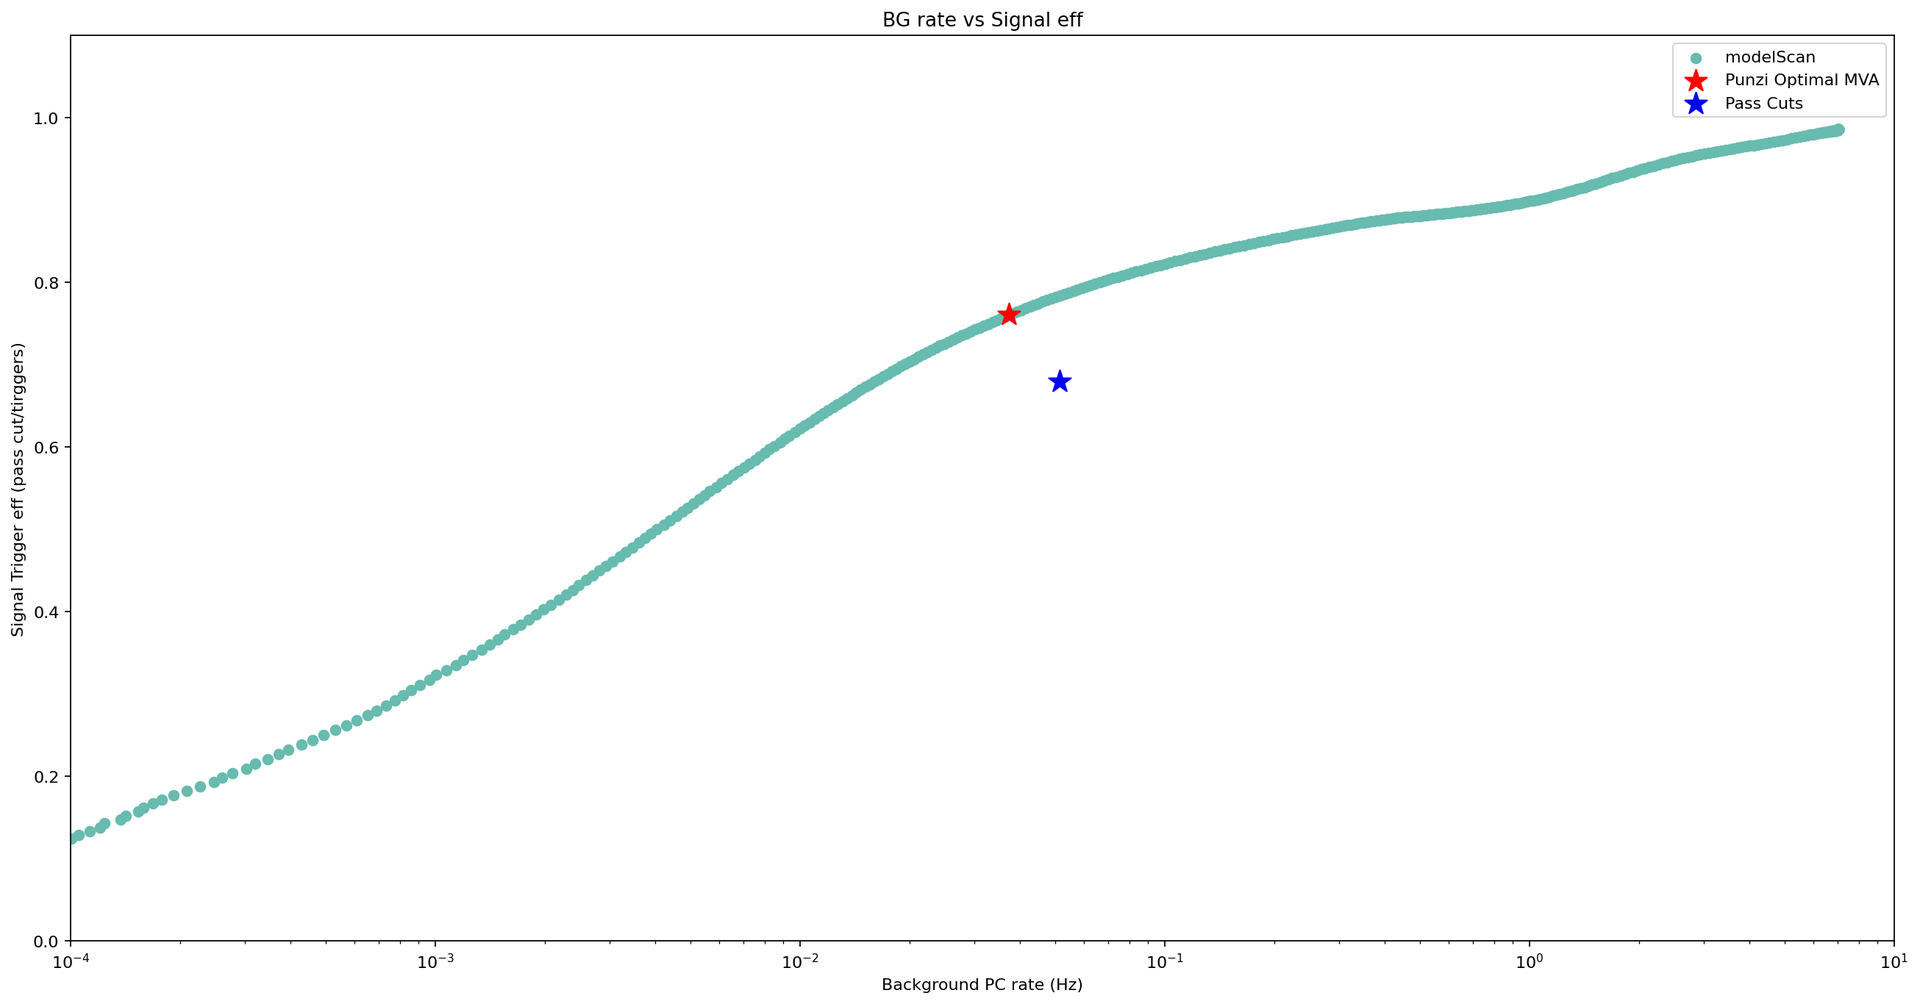
\includegraphics[width = \textwidth]{figures/chapter 4/MVA-punzi.png}
\caption{MVA scan plot. The cyan curve represents scan of the MVA model varying the selection criteria. The red star is the optimal point corresponding to the minimization of the Punzi figure of merit \cite{punzi2003sensitivitysearchesnewsignals}. The MVA curve is obtained by training the algorithm on data without \Hbar trapped, recording only annihilations from muons, and annihilations recorded during the mixing phase, during which the background is negligible and events are mainly constituted by un-trapped \Hbar .}
\label{fig:MVAscan}
\end{figure}

The cosmic background corresponding to the red star is the chosen working point, and the data that will be presented are related to that particular selection criterion. The signal efficiency rate is 75.7(5) \%, and the background is \SI{37.4(7)}{ \milli \hertz}. 
Although these quoted values are estimated from runs with several thousand recorded events, the actual background during the experimental runs can be different. Due to the presence of electrode heating, a portion of the atoms could annihilate on residual gas. The amount of gas present in the trap is not controlled, hence the background is a free parameter in the analysis, and has not been fixed to the expected value from the MVA selection.

\section{Signal Model Definition}

%In the analysis model, it is used for the {\it frequency marker} a definition related to the onset of the transition. With respect to previous measurement \cite{ALPHA:2017fsh}, however, some modifications are necessary, to account for the increased $\overline{\mathrm{H}}$ population in each run (which may result in detectable background from anti-atoms escaping the trap for reasons different than microwave-induced spin-flips) and for the increased sensitivity to differences between the \cb and \da lineshapes. 

The lineshape model $f(\cdot)$ for the fit of the experimental data is constructed as the convolution of two functions: a bare function $g(\cdot)$ and a resolution/broadening function $R(\cdot)$:

\begin{equation}
\centering
f \equiv g \otimes R \,.
\label{eq:conv}
\end{equation}

The bare function $g$ is introduced to describe the energy distribution, magnetic field profile, and depletion effects which determine the lineshape. It has a well-defined onset of the transition, and an exponentially decaying right tail. The resolution function has been introduced to describe all those effects that are related to broadening of the resolution conditions, such as magnetic field inhomogeneities, magnetic field fluctuations, Doppler broadening, and transit-time broadening.
The function has been expressed in terms of a parameter that describes the frequency position of the \cb and \da lineshapes, and acts therefore as a \textit{frequency marker} ($f_o$). Although tempting, these frequency markers are only related to the resonance frequency at a given condition, because of several broadening effects that will be discussed later in this chapter. The difference of the frequency markers for the \cb and \da transitions, corrected for the magnetic field decay, is an estimate of the antihydrogen hyperfine splitting frequency $a_{1S}/h = f_o^{(da)} - f_o^{(cb)}$. 
The actual shape of $g$ cannot be derived directly from first principles, since it would require knowledge of the microwave standing wave pattern, the actual power delivered to the trap, and the energy distribution of the atoms. These quantities are not known with enough precision, hence the signal model corresponds to an empirical function which satisfies the following requirements:

\begin{itemize}
    \item its value is zero for frequency values lower than $f_o$, and strictly positive for frequencies higher than  $f_o$; 
    \item it features a monotonic rise (corresponding to an increase in the resonant volume as the frequency is increased) between $f_o$ and the maximum of the function;
    \item it features a monotonic decay (associated to the decreasing antihydrogen population as the scan progresses) after the maximum.
\end{itemize}

The bare function $g$ is described by Eq.~\ref{eq:model1}:

\begin{equation}
\centering
g(\overline{x})=
\begin{dcases}
 0        & \overline{x} < - \sigma (k + 1) \\
\exp\left(-\frac{1}{2}\right) \times \left[\frac{\overline{x} + \sigma (k + 1)}{\sigma k}\right]^k  & [\overline{x} > - \sigma (k + 1)] \land (\overline{x}<- \sigma) \\
\exp\left(-\frac{\overline{x}^2}{2\sigma^2}\right)  & (\overline{x} >-\sigma) \land (\overline{x}<0) \\
\exp\left(-\frac{\overline{x}^2}{2\sigma_r^2}\right) & (\overline{x} >0) \land (\overline{x}< \sigma_r) \\
\exp\left(-\frac{1}{2}\right)\left[\frac{\overline{x} + \sigma_r(n-1) } {\sigma_rn} \right]^{-n} & \overline{x} > \sigma_r \\
\end{dcases}
\label{eq:model1}
\end{equation}

The onset (our chosen frequency marker) is defined as the minimum value at which the above equation differs from zero, while the function parameters have the following meaning:

\begin{itemize}
    \item $\overline{x} \equiv x - x_{max}$. Therefore, $\overline{x} = 0$ is the position of the maximum;
    \item $\sigma$ is the standard deviation for the left-side Gaussian-like component;
    %    \item $-b\sigma$ represents the connection point between the polynomial rise and the Gaussian;
    \item $k$ is the degree of the polynomial describing the rise portion; 
    %\item $r = \sigma \cdot \frac{k + b^2}{b}$ 
    %    \item $C= \exp(-\frac{b^2}{2})$ ensures the continuity in the function;
    \item $r = \sigma \cdot (k + 1)$ is the distance (rise length) between the onset and the maximum;
    %\item $a$ describes the weight of the right-side non-Gaussian tail;
    \item $\sigma_{r}$ is the  standard deviation of the right-side Gaussian core portion, while $n$ describes the power-law right-tail (Crystal Ball function).  
\end{itemize}

Although complex, the core of this model has been developed considering a power law rise to describe the early part of the lineshape, and an asymmetric tail to describe the later part of the lineshape, and imposing continuity and first-order differentiability at the junction point.
To gain some physical intuition on the model, one can think of the bare function $g$ as describing the lineshape we would observe if the atoms were stationary, the microwave radiation monochromatic, the magnetic field perfectly stable, etc., i.e., if all broadening sources were turned off. 

In this hypothetical case, for an upward microwave frequency ramp, the onset would be well defined: it would correspond to the infinitely-large sample-size limit of the minimum value corresponding to the first significant annihilation count, and would be associated with the lowest value of the magnetic field. In practice, since the experiment is not dealing with stationary atoms and a perfect magnetic field, a certain level of broadening is expected.

\subsubsection{The resolution/broadening function} \label{sec:resolutionF}

Simulations show that spin-flip transitions can occur at frequencies lower than the frequency corresponding to the magnetic field minimum, due to effects such as: 
\begin{itemize}
    \item \textbf{Fluctuations in the magnetic field.} The resonance condition is set by the magnetic field at the trap minimum, and near \SI{1}{\tesla} the positron spin-flip frequencies change by about \SI{28}{\giga\hertz} per tesla \cite{ALPHA:2026lbu}. A field change as small as \SI{0.4}{\micro\tesla}, less than one part per million of the bias field, therefore moves the resonance by about \SI{10}{\kilo\hertz}. The currents in the trap magnets are actively stabilized to within a few mA, but small residual fluctuations and short glitches remain (Sec.~\ref{sec:DCCTs}): whenever the field at the minimum is momentarily lower, atoms can come into resonance at a microwave frequency below the nominal onset.
    \item \textbf{Width of the microwave radiation in the trap.} The radiation is produced by a synthesizer referenced to a \SI{10}{\mega\hertz} signal provided by CERN, so the intrinsic spectral width of the injected radiation is negligible compared with the \SI{5}{\kilo\hertz} frequency step \cite{ALPHA:2026lbu}; annihilations occurring while the synthesizer settles to a new frequency ( $\approx$ \SI{30}{\milli\second} after each step) are vetoed. More relevant is the fact that the radiation reaches the atoms through the electrode stack as a superposition of standing and travelling waves, whose amplitude and polarization change with position. An atom therefore experiences a microwave field whose strength varies along its trajectory, which mainly affects the transition rate, as discussed below for power broadening.
    \item \textbf{Doppler-shift broadening.} An atom moving along the propagation direction of the radiation sees the microwave frequency shifted by a fraction $v_z/c$. For the energies of the trapped atoms (below \SI{0.5}{\kelvin}) this shift is a few kHz, as estimated in Sec.~\ref{sec:Doppler}. Since the frequency is scanned from below, only the atoms that see the radiation shifted upwards matter, as they come into resonance before the nominal onset; the resulting contribution is therefore one-sided.
    \item \textbf{Transit-time broadening.} An atom does not sit at the field minimum, but moves through the trap, and stays in resonance only for the short time it takes to cross the region where its detuning is small. A transition driven for a finite time $\tau$ is not sharp in frequency, but has a width of order $1/\tau$: for example, an effective interaction time of \SI{0.1}{\milli\second} corresponds to a width of about \SI{10}{\kilo\hertz}. Atoms crossing the minimum can therefore undergo a spin flip even if the microwave frequency is slightly below the resonance frequency at the minimum.
    \item \textbf{Power broadening.} A stronger microwave field drives the spin flip faster, and the range of detunings over which a transition can still occur becomes wider, roughly in proportion to the amplitude of the oscillating magnetic field (the Rabi frequency). This effect is visible in the simulations, where the fitted broadening increases with the microwave field amplitude (Tab.~\ref{tab:resfun}). Since the power that reaches the atoms depends on frequency, it can differ between the two transitions: this is why the injected powers are balanced (Sec.~\ref{sec:MWpower}), and why the residual difference is included in the systematic uncertainty.
\end{itemize}

Transit-time and power broadening are included in the simulations, which compute the spin-flip probability along each trajectory with a time-dependent detuning \cite{ALPHA:2026lbu}, while the Doppler effect is not, and is estimated separately (Sec.~\ref{sec:Doppler}).

Estimating the size of these effects from simulations or calculations is expected to be an easier task than simulating the full lineshape, at least under a set of reasonable simplifying assumptions. Therefore, we describe such broadening effects in the model by convolving the bare function $g$ with the resolution function $R$. The parameters of the resolution function are determined from simulations and calculations, and are fixed in the fit to the \Hbar data, i.e., there are no floating parameters associated with the resolution function in the fit to the data.

Since monotonic upward frequency scans are performed in the experimental runs, the broadening function is one-sided. This choice assumes that a negligible portion of the atoms whose frequency matches the microwave frequency during the scan will evade transition. This could apparently conflict with the fact that a certain amount of atoms do not undergo a transition, and are finally ejected during the \textit{clearing} scan. However, there are physical mechanisms that can explain this: in fact, the evidence from the simulation indicates that the trajectories of antihydrogen atoms are chaotic. Hence, even though during the scan a certain resonant volume is depleted, it is not assured that some of the atoms won't repopulate a specific resonant volume further during the scan.

The approach followed in this analysis uses a resolution function whose shape and width can be varied to determine systematic uncertainties. The simulations were used to test different combinations of bare function $g$ and broadening function $R$.
The broadening function might depend on the step in the scan (i.e., might vary with frequency), but we can assume that the only part affecting the zero frequency marker is the one evaluated at the first significant step. 

The broadening may also depend on the population kicked out in the first step, which might in principle differ between the two transitions. % (i.e., there is a dependence on power); 

Even if the two broadening functions were the same, a different underlying bare function would result in a different effect on the {\it frequency marker}, which wouldn't cancel in the difference between the two transitions. 

We can assume different shapes for the broadening function, such as a one-sided Gaussian or a one-sided cusp. A right-sided tail (of negligible width, $t_R = 0.2\,{\rm kHz}$, compared to the frequency step) is included for numerical stability. For a Gaussian we have: 

\begin{equation}
\centering
R(\overline{x})=
\begin{dcases}
 \exp\left(-\frac{1}{2}\frac{x^2}{t_{gauss}^2}\right)        & x < 0 \\
 0 & x \geq 0\\
% \exp\left(-\left|\frac{x}{t_R}\right|\right)        & x \geq 0 \\
\end{dcases}
\label{GaussR}
\end{equation}
while for a one-sided cusp:
\begin{equation}
\centering
R(\overline{x})=
\begin{dcases}
 \frac{1}{t_{cusp}}\exp\left(-\frac{x}{t_{cusp}}\right)        & x < 0 \\
0        & x \geq 0 \\
\end{dcases}
\label{CuspR}
\end{equation}

An example of the bare function $g$ and of its convolution with the resolution function, fitted to the first repetition of a dataset, is shown in Fig.~\ref{fig:ModelVsData}.

\begin{figure}[!hbtp]
\centering
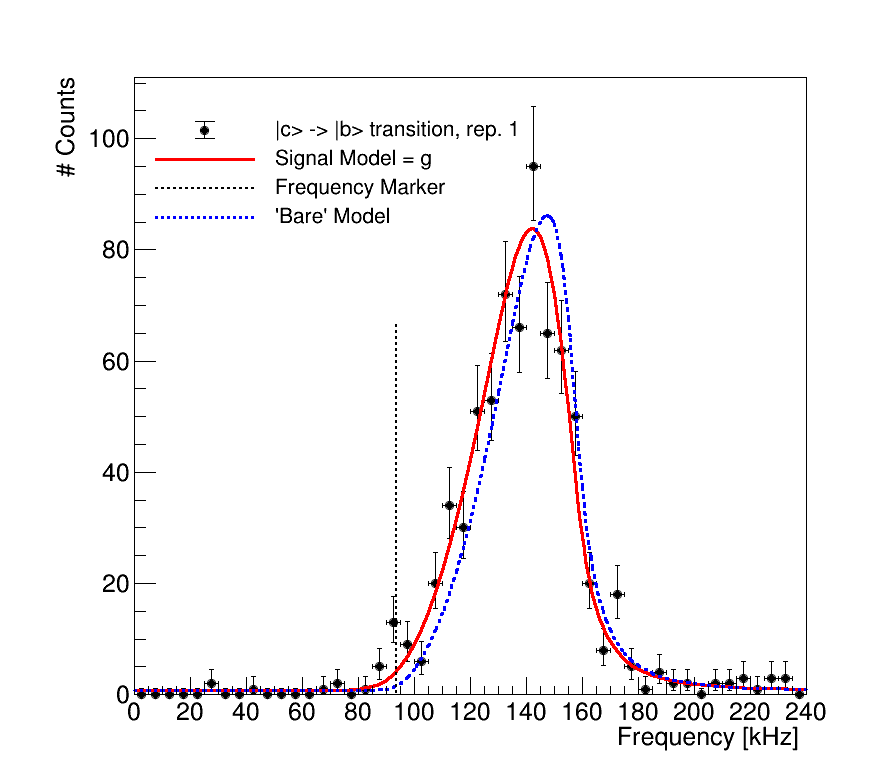
\includegraphics[width = \textwidth]{figures/chapter 4/Model_vs_data_s8.png}
\caption{Lineshape of the first repetition of the low field (\SI{1.03}{\tesla}) dataset. The blue line represents the bare function $g$ with best fit parameters. The red line represents the bare function $g$ convoluted with the resolution function (one-sided Gaussian with \SI{10}{\kilo\hertz} standard deviation), the black vertical dotted line is the frequency marker or onset position.}
\label{fig:ModelVsData}
\end{figure}

\section{Simulation} \label{sec:Simulation}

\contentof{In this section explain the simulation and how it has been used to estimate the systematic. The shown the plot of the simulation lineshapes and describe the limits of the simulation.}

Simulations of the experiment, involving antihydrogen motion and its interaction with microwaves, have been conducted to inform the model parameters and study some of the systematics of the measurement. The simulation reflects the experimental protocol, following the magnet manipulations and the frequency ramps. The magnetic field has been tuned using ECR data, the ones shown in Fig.~\ref{fig:flatfield}.

The simulation cannot describe the experiment with the required precision because of the lack of knowledge of the magnetic field off-axis and the unknown microwave field pattern in the trap. Therefore, the simulation has been used to inform the signal model parameters, such as the degree of the power-law rise of the lineshape. Different lineshapes corresponding to different microwave powers are available (Fig.~\ref{fig:SimLineshapes}), and have been fitted with the current signal model. Based on these fits (Tab.~\ref{tab:resfun}), the degree of the power-law rise has been fixed to $k=2$ in the nominal analysis, and the broadening parameters to $t^{cb}_{gauss} = t^{da}_{gauss} = \SI{10}{\kilo\hertz}$, half-way between the results obtained for the 2023 and 2024 simulations.

\begin{figure}[!hbtp]
\centering
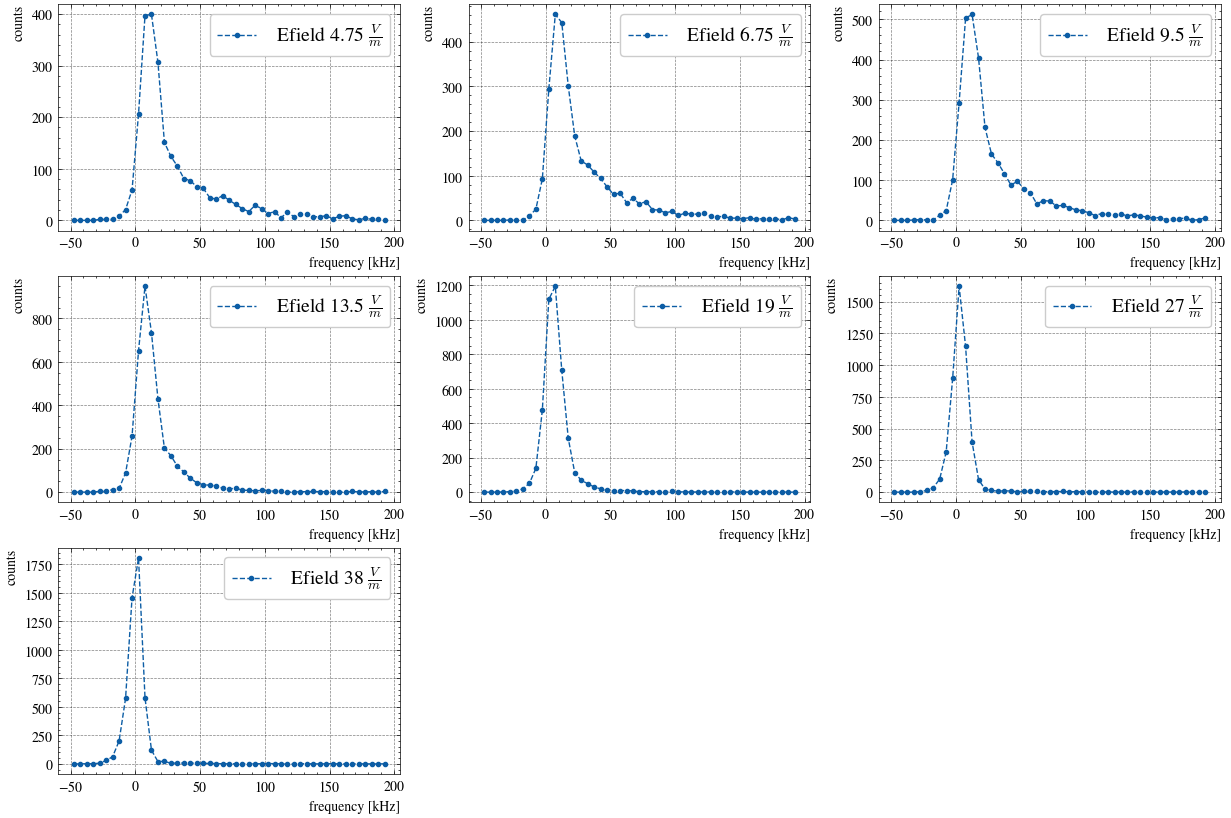
\includegraphics[width=\textwidth]{figures/chapter 4/FrancisSimulation_2024.png}
\caption{ Simulation of microwave induced annihilation for different electric field amplitudes (in legend reported as \SI{}{\volt\per\meter}). The simulation does not account for differences in the standing wave pattern for the \cb and \da transitions; consequently, the simulated \da lineshape is essentially identical to the \cb one, aside from the frequency offset corresponding to the splitting.}
\label{fig:SimLineshapes}
\end{figure}



\section{Maximum Likelihood Fit} \label{sec:MLEfit}

The analysis approach to extract the splitting from the raw data has been developed using the frequentist framework, where the best-fit parameters result from the maximization of the likelihood function \likelihood. As mentioned in Sec.~\ref{sec:Protocol}, the data are divided into two sets of eight repetitions, each consisting of a single \cb and \da transition measurement interspersed with stacking phases. Details of the specific runs and available data are reported in Tab.~\ref{tab:ListOfRuns}. 

\begin{table}[!ht]
    \centering
    \begin{tabular}{l|cccc}
         \hline\hline
% SERIES 7 ___________________
      {\bf \SI{1.07}{\tesla} dataset} & & & & \\
          {\bf Carlsberg reset}  & \multicolumn{3}{l}{19 May 2024: reset to 194.358 A} & 12:40     \\
    {\bf Repetition}   & {\bf Run}  & {\bf cb Init Freq (kHz)} & {\bf Unix Time (s)} & {\bf Time}  \\
          \hline

         
         0              &   70377   &$29\,418\,364$	 & 1716123393.873294	& 14:03 \\ 
         1              &   70378   &$29\,418\,284$	 & 1716129652.988256	&  \\ 
         2              &   70379   &$29\,418\,187$	 & 1716135002.727111	&  \\
         3              &   70380   &$29\,418\,073$	 & 1716140853.490512	&  \\ 
         4              &   70381   &$29\,417\,956$	 & 1716146112.077295	&  \\ 
         5              &   70382   &$29\,417\,741$	 & 1716155966.214942    &  \\ 
         6              &   70383   &$29\,417\,607$	 & 1716162057.169858    &  \\
         7              &   70384   &$29\,417\,488$  &  1716167889.394672	&  \\
         \hline
         (bkg study)    &   70385   &                &  	                &  \\
         post           &   70386   & $29\,416\,964$ & 1716193095.703465    & 10:48 (+1d) \\
         \hline
         \hline
% SERIES 8 ___________________
         {\bf \SI{1.03}{\tesla} dataset} & & & & \\
         {\bf Carlsberg reset} & \multicolumn{3}{l}{23 May 2024: reset to 186.426 A} & 13:13 \\
         {\bf Repetition}      & {\bf Run}  & {\bf cb Init Freq (kHz)} & {\bf Unix Time (s)} & {\bf Time} \\
          \hline 
         0            & 70462   & $28\,227\,463$	&	1716497309.208071	& 22:38 \\ 
         1            & 70463   & $28\,227\,387$	&	1716502378.209453	& \\ 
         2            & 70464   & $28\,227\,231$	&	1716509895.094319	& \\
         3            & 70465   & $28\,227\,132$    &	1716514501.176821	& \\ 
         4            & 70467   & $28\,226\,914$	&	1716524509.825337	& \\   
         5            & 70468   & $28\,226\,811$	&	1716529827.672246	& \\
         6            & 70469   & $28\,226\,710$	&	1716534513.851191	& \\
         7            & 70470   & $28\,226\,613$	&	1716539621.420382	& \\
         \hline
         pre          & 70461   & $28\,227\,609$	&	1716492680.251725	& 21:28       \\
         post         & 70471   & $28\,226\,227$    &	1716558788.451213	& 15:53 (+1d) \\
       \hline
       \hline
    \end{tabular}
    \caption{List of runs used in the analysis of the two datasets at lower and higher B-field. The initial frequency of the \da scan is set $1\,420\,390\,{\rm kHz}$ above the initial frequency of the \cb scan.}
    \label{tab:ListOfRuns}
\end{table}

The time interval between a run and the next one is \SI{1}{\hour} during which antihydrogen is accumulated in the trap by repeating mixing cycles of 4 minutes each. The total number of atoms accumulated for each run is $1400-1600$, equally split between the c and d states. The Maximum Likelihood fit consists in analysing the data simultaneously, with a likelihood defined as the sum of the individual likelihoods for each repetition:

\begin{equation}
\mathcal{L}_{tot} = \sum_{cb;da} \sum_{i} \mathcal{L}_{i}(\vec{\mu}, \vec{x})
\end{equation} 

Where $\vec{\mu}$ is the parameter space and $\vec{x}$ are the observations. The total likelihood is the sum of the likelihoods of each individual spectrum, and the minimization acts on the total likelihood. The advantage of this shared minimization is that the model complexity can be reduced, since some of the parameters are shared among repetitions of the same transition, increasing the statistical power for the fit of the shape parameters and improving the fit minimization. In the nominal analysis, the parameters controlling the shape of the spectra ($\sigma, \sigma_{r}, n_{r}$) are shared among repetitions of the same transition, while the normalization $nS_{i}$, the background, and the frequency markers $f_{cb,da;i}$ are individual for each repetition. As an example, the result of the fit for a single repetition is shown in Fig.~\ref{fig:ExampleSpectra}.

\begin{figure}[!hbtp]
\centering
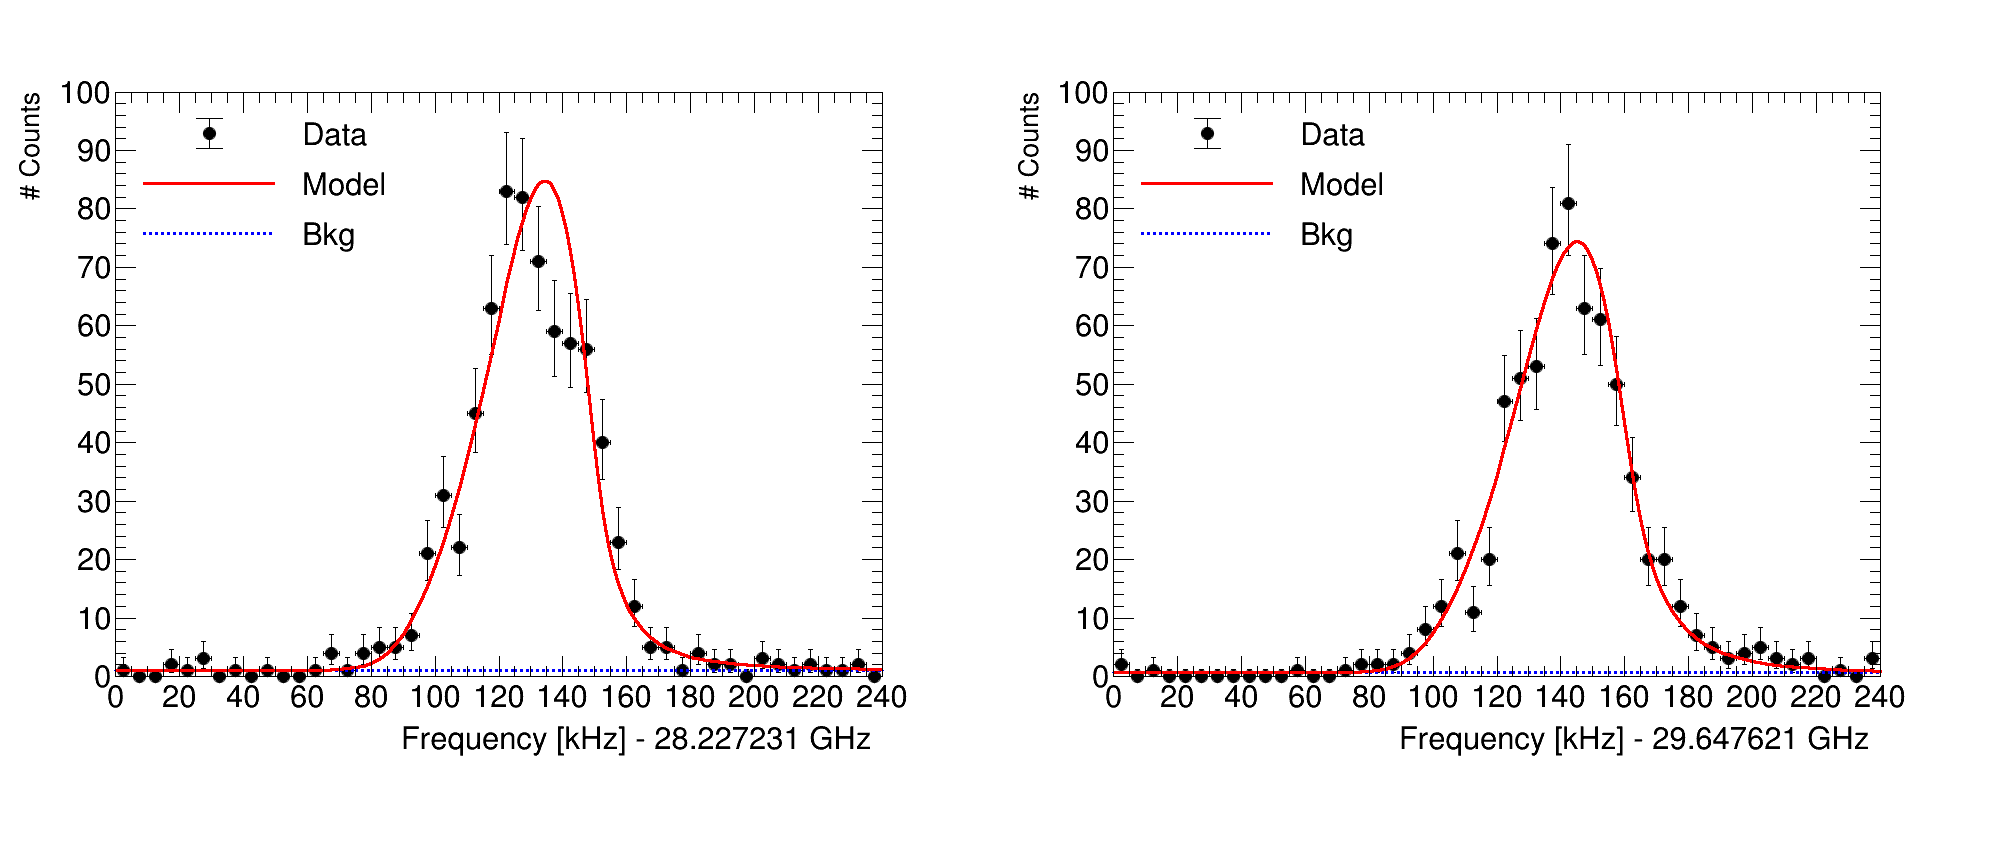
\includegraphics[width=\textwidth]{figures/chapter 4/Example-of-spectra.png}
\caption{Result of the maximum likelihood fit on repetition 3 for the set at \SI{1.03}{\tesla}.}
\label{fig:ExampleSpectra}
\end{figure}

\subsection{Blinding the Analysis}

The analysis was conducted blind to avoid bias during the development. A random offset $\delta f_{blinding}$ value was added to all frequency markers of the \da transition, applied uniformly across both datasets.

\begin{equation} \label{eq:deltaf}
f_{da}^{i} \equiv  f_{da}^{i} (t_{i}) +  \delta f_{blinding}
\end{equation}

Consequently, the hyperfine splitting extracted from both series was shifted by the same unknown quantity. This offset was revealed only when all the systematic uncertainties had been determined and a common consensus of the analysis procedure had been reached among ALPHA collaboration members.

Throughout this chapter the following convention is adopted. Absolute values of the hyperfine splitting quoted in tables (Tabs.~\ref{tab:results}, \ref{tab:selections}, \ref{tab:highstat_floatk}, \ref{tab:highstatparam}) are blind, and do not include the separation of \SI{1420390}{\kilo\hertz} between the \cb and \da sweeps. Quantities that are differences between analysis configurations ($\Delta$ columns, Tab.~\ref{tab:syst}), residuals and drift slopes (Tab.~\ref{tab:resultsBdrift}) do not depend on the blinding offset. Values quoted in full (e.g.\ $1\,420\,404.8$~kHz) are unblinded.

\subsection{Correlation between observables} \label{sec:Correlation}

The combined maximum likelihood estimation (MLE) approach, in which the model $f = g \otimes R$ of Eq.~\ref{eq:conv}, with the bare function $g$ of Eq.~\ref{eq:model1} and the resolution function $R$ of Eq.~\ref{GaussR}, is fitted simultaneously to all the repetitions of a series, offers several advantages. First, it reduces model complexity by allowing certain parameters to be shared across different datasets rather than fitted independently for each. Second, shape parameters like $\sigma_{rise}$ and $n_r$ benefit from the increased statistical power, as a consequence of being treated as global parameters. On the other hand, this approach introduces correlations between parameters, in particular the frequency markers, that must be carefully accounted for when deriving statistical uncertainties. Fig.~\ref{fig:CorrelationHeatMap} shows the correlation heat map of the MLE fit of the low-field series. As evident from the map, $\sigma_{cb}$ and $\sigma_{da}$, which control the onset shape of the spectra, are correlated with the frequency markers. This correlation arises because the shape parameters are constrained to be identical across repetitions, which in turn constrains the fitted frequency markers. The resulting covariance matrix of the frequency markers is reported in Tab.~\ref{tab:cov_matrix}.

\begin{figure}[!hbtp]
\centering
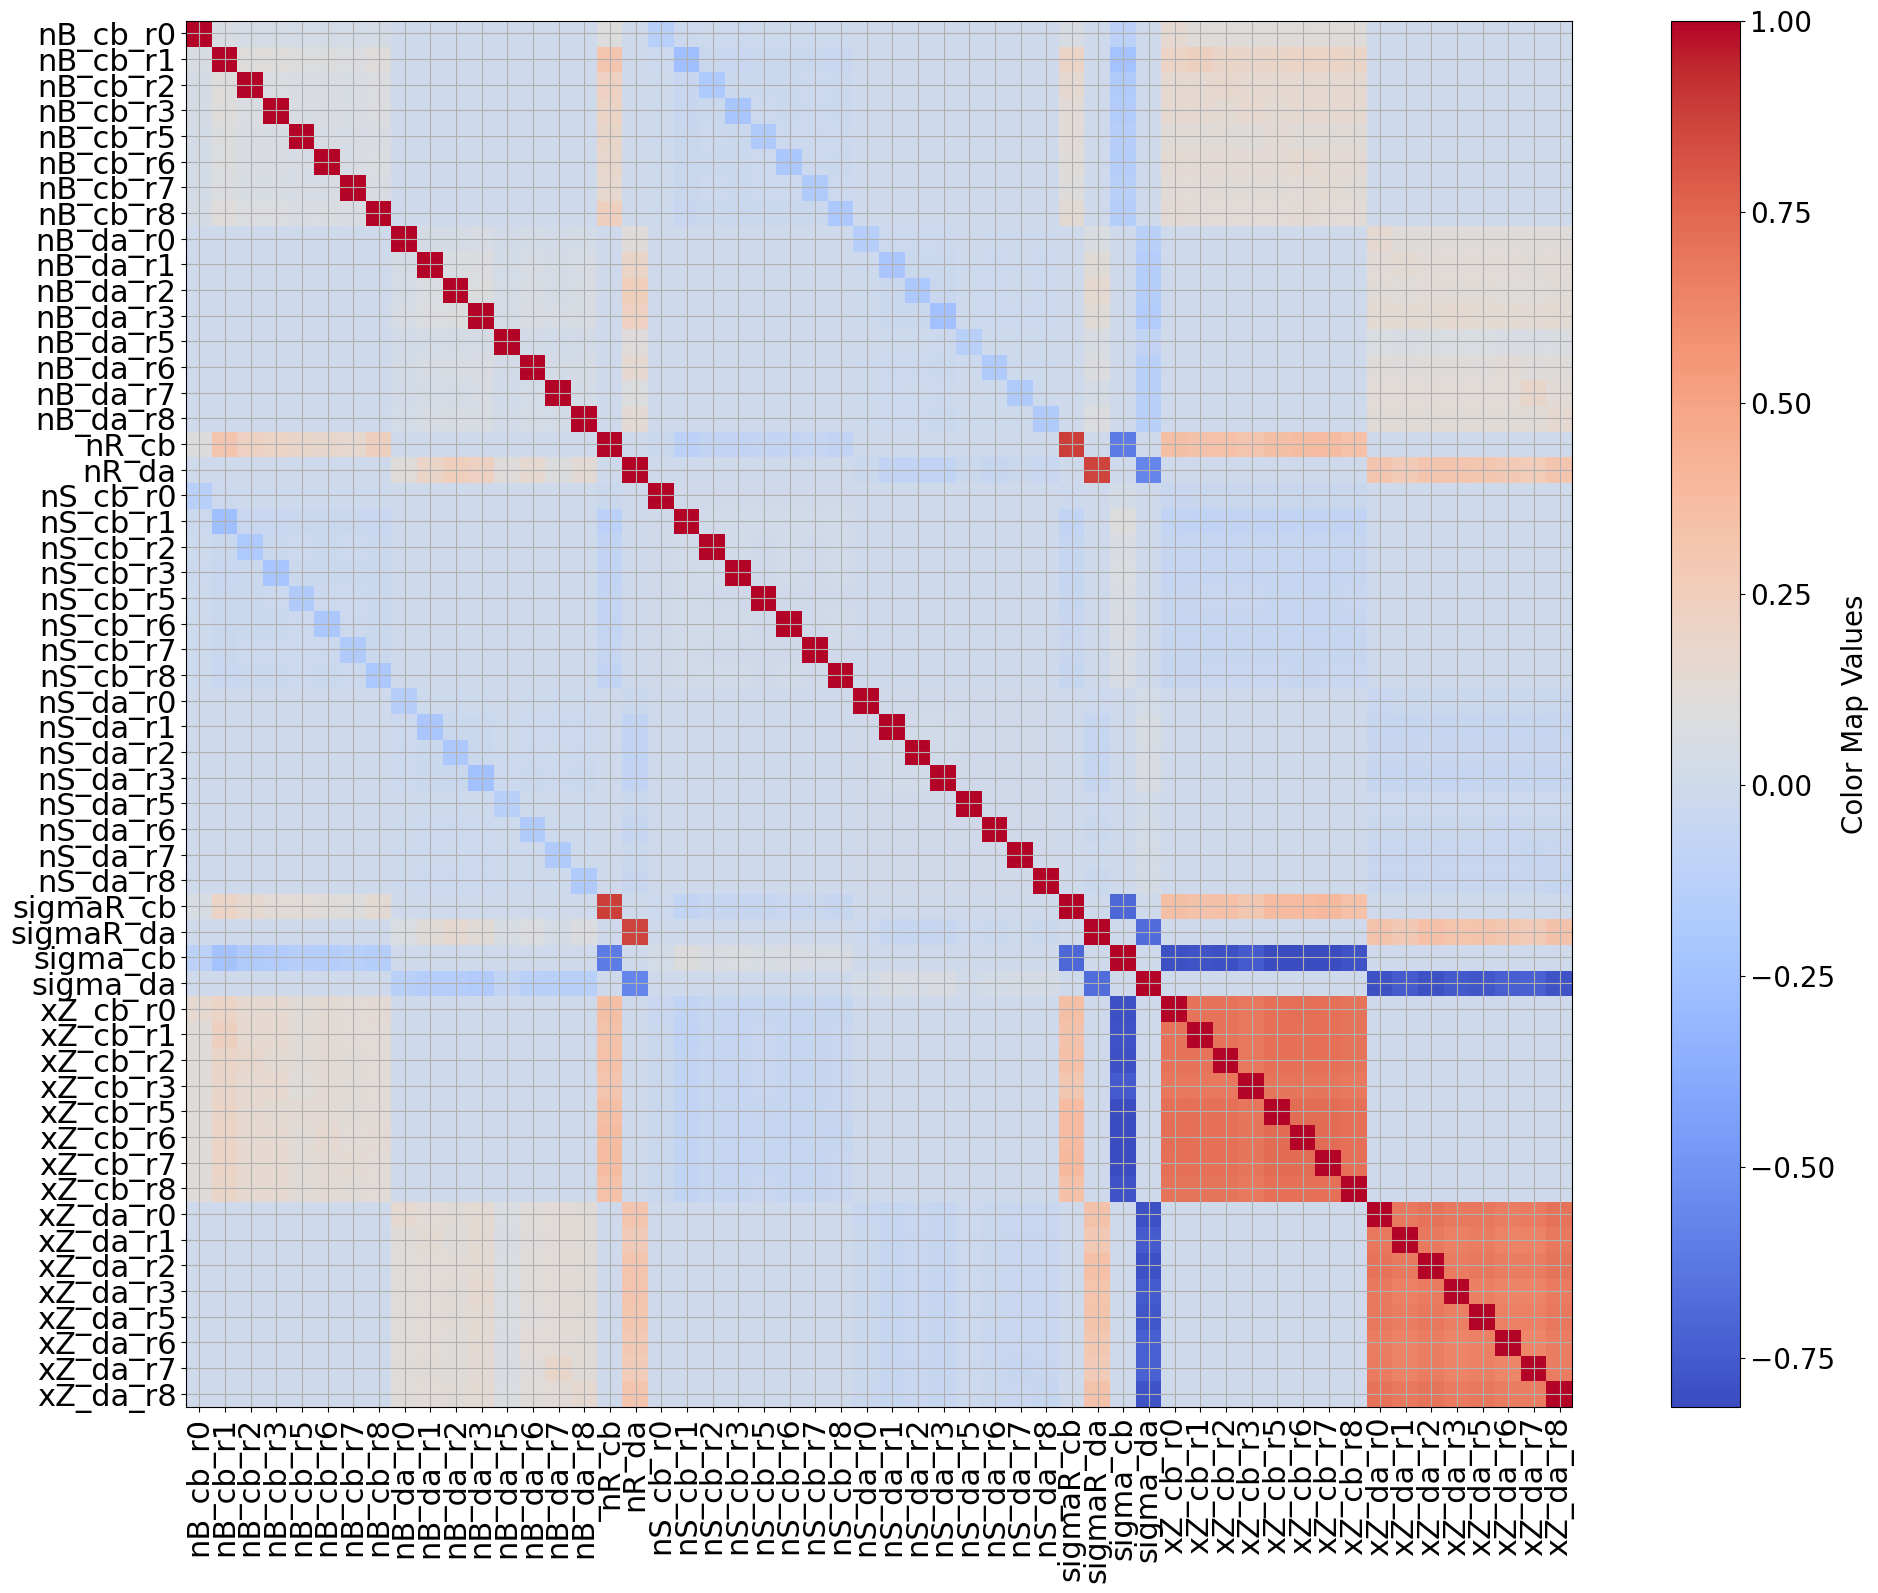
\includegraphics[width =  \textwidth]{figures/chapter 4/correlation_matrix_2026-05-28 102938_s8.png}
\caption{Correlation matrix of the MLE fit for the set of data at \SI{1.03}{\tesla}. The block of parameters labelled \texttt{xZ\_xx\_ry}, where \texttt{xx} denotes the transition (\texttt{cb} or \texttt{da}) and \texttt{y} the repetition number, corresponds to the frequency markers (the nomenclature used in the analysis code). The correlation of the frequency markers within the same transition is evident, as is their correlation with the shape parameter $\sigma_{xx}$. Correlations are also observed among other shape parameters $\sigma_{R,xx}$ and $n_{r,xx}$. These do not pose a problem since they influence the depletion tail of the spectrum, and are insensitive to the onset position.}
\label{fig:CorrelationHeatMap}
\end{figure}

\begin{table}[h]
    \centering
    \small 
    \scalebox{0.75}{
    \renewcommand{\arraystretch}{1.2}
    \begin{tabular}{l|cccccccc|cccccccc}
    \hline \hline
    & \multicolumn{8}{c|}{$f_{cb}$} & \multicolumn{8}{c}{$f_{da}$} \\
    \hline
\multirow{8}{*}{$f_{cb}$} & 2.23 & 1.36 & 1.34 & 1.41 & 1.40 & 1.40 & 1.31 & 1.40 & 0.00 & 0.00 & 0.00 & 0.00 & 0.00 & 0.00 & 0.00 & 0.00 \\
& 1.36 & 2.16 & 1.33 & 1.39 & 1.38 & 1.39 & 1.29 & 1.39 & 0.00 & 0.00 & 0.00 & 0.00 & 0.00 & 0.00 & 0.00 & 0.00 \\
& 1.34 & 1.33 & 2.23 & 1.38 & 1.37 & 1.38 & 1.29 & 1.38 & 0.00 & 0.00 & 0.00 & 0.00 & 0.00 & 0.00 & 0.00 & 0.00 \\
& 1.41 & 1.39 & 1.38 & 2.32 & 1.44 & 1.44 & 1.35 & 1.44 & 0.00 & 0.00 & 0.00 & 0.00 & 0.00 & 0.00 & 0.00 & 0.00 \\
& 1.40 & 1.38 & 1.37 & 1.44 & 2.37 & 1.43 & 1.33 & 1.43 & 0.00 & 0.00 & 0.00 & 0.00 & 0.00 & 0.00 & 0.00 & 0.00 \\
& 1.40 & 1.39 & 1.38 & 1.44 & 1.43 & 2.13 & 1.34 & 1.44 & 0.00 & 0.00 & 0.00 & 0.00 & 0.00 & 0.00 & 0.00 & 0.00 \\
& 1.31 & 1.29 & 1.29 & 1.35 & 1.33 & 1.34 & 2.11 & 1.34 & 0.00 & 0.00 & 0.00 & 0.00 & 0.00 & 0.00 & 0.00 & 0.00 \\
& 1.40 & 1.39 & 1.38 & 1.44 & 1.43 & 1.44 & 1.34 & 2.28 & 0.00 & 0.00 & 0.00 & 0.00 & 0.00 & 0.00 & 0.00 & 0.00 \\
\hline
\multirow{8}{*}{$f_{da}$} & 0.00 & 0.00 & 0.00 & 0.00 & 0.00 & 0.00 & 0.00 & 0.00 & 2.36 & 1.50 & 1.46 & 1.48 & 1.40 & 1.44 & 1.43 & 1.51 \\
& 0.00 & 0.00 & 0.00 & 0.00 & 0.00 & 0.00 & 0.00 & 0.00 & 1.50 & 2.04 & 1.39 & 1.41 & 1.33 & 1.37 & 1.36 & 1.44 \\
& 0.00 & 0.00 & 0.00 & 0.00 & 0.00 & 0.00 & 0.00 & 0.00 & 1.46 & 1.39 & 2.16 & 1.38 & 1.31 & 1.34 & 1.33 & 1.40 \\
& 0.00 & 0.00 & 0.00 & 0.00 & 0.00 & 0.00 & 0.00 & 0.00 & 1.48 & 1.41 & 1.38 & 2.14 & 1.32 & 1.36 & 1.34 & 1.42 \\
& 0.00 & 0.00 & 0.00 & 0.00 & 0.00 & 0.00 & 0.00 & 0.00 & 1.40 & 1.33 & 1.31 & 1.32 & 2.11 & 1.29 & 1.28 & 1.35 \\
& 0.00 & 0.00 & 0.00 & 0.00 & 0.00 & 0.00 & 0.00 & 0.00 & 1.44 & 1.37 & 1.34 & 1.36 & 1.29 & 1.88 & 1.31 & 1.39 \\
& 0.00 & 0.00 & 0.00 & 0.00 & 0.00 & 0.00 & 0.00 & 0.00 & 1.43 & 1.36 & 1.33 & 1.34 & 1.28 & 1.31 & 1.97 & 1.37 \\
& 0.00 & 0.00 & 0.00 & 0.00 & 0.00 & 0.00 & 0.00 & 0.00 & 1.51 & 1.44 & 1.40 & 1.42 & 1.35 & 1.39 & 1.37 & 2.16 \\
\hline
    \end{tabular}
    }
    \caption{Covariance matrix of the frequency markers. The values in the off-diagonal blocks are of the order of $10^{-4}$--$10^{-5}$; the values have been written with a precision of 2 decimal places.}
    \label{tab:cov_matrix}
\end{table}

\subsection{Maximum Likelihood Fit: Results}

The results of the nominal maximum likelihood fit for the two series are summarized in Tab.~\ref{tab:resultsf0}. Two parameters are kept fixed in the nominal configuration: the width of the one-sided Gaussian resolution function, $t_{gauss} = \SI{10}{\kilo\hertz}$ for both transitions, obtained from the fit to the simulations (Sec.~\ref{sec:Simulation}), and the degree of the power-law rise, $k=2$. The shape parameters of the bare function $g$ ($n$, $\sigma$, $\sigma_r$) are shared among the eight repetitions of the same transition, but are determined separately for the \cb and \da transitions. The table also reports the corresponding rise length $r = \sigma (k+1)$, i.e.\ the distance between the onset and the maximum of the lineshape, and the sixteen frequency markers of each series, one for each repetition and transition. Since each spectrum is fitted after setting the first frequency of its scan to zero, the markers are expressed relative to the initial frequency of the corresponding scan; the initial frequencies of the \cb and \da scans of the same repetition are separated by \SI{1420390}{\kilo\hertz} (Tab.~\ref{tab:ListOfRuns}). The \da markers are reported after unblinding, i.e.\ with $\delta f_{blinding} = 0$.

Some features of the results are worth noting. The parameters that control the onset region of the lineshape are very similar for the two transitions: $\sigma$ is about \SI{19}{\kilo\hertz} in the high-field series and \SIrange{20}{21}{\kilo\hertz} in the low-field series, and the rise lengths of the \cb and \da transitions agree within about one standard deviation in both series. This indicates that the balancing of the microwave power between the two transitions (Sec.~\ref{sec:MWpower}) was effective where it matters most, since the onset region is the part of the spectrum that determines the frequency markers. Larger differences between the two transitions are found in $\sigma_r$ and $n$, which describe the depletion tail of the lineshape and, as discussed in Sec.~\ref{sec:Correlation}, are only weakly correlated with the frequency markers. The statistical uncertainty of each marker is \SIrange{1.2}{1.5}{\kilo\hertz}; part of it comes from the shared shape parameters, which also produce the correlations between the markers of the same transition shown in Tab.~\ref{tab:cov_matrix}.

The markers change from one repetition to the next, since the initial frequency of each scan is set according to the expected magnetic field drift (Fig.~\ref{fig:RepetitionScheme}), and the actual drift differs from the expected one. Moreover, the \da scan starts about \SI{812}{\second} after the \cb scan of the same repetition, during which the magnetic field keeps decaying. For these reasons, the difference $f_{o,da}^{(i)} - f_{o,cb}^{(i)}$ of a single repetition is not directly an estimate of the hyperfine splitting: the markers must first be corrected for the magnetic field drift, as described in the next section.

% TABLE 6 - RESULTS
\begin{table}[!h]
\centering
\begin{tabular}{l|cc}
\hline
\hline
\textbf{} & \textbf{\SI{1.07}{\tesla} (high field)}  &  \textbf{\SI{1.03}{\tesla} (low field)}  \\
\hline 
$t_{gauss}^{(cb)}$ (kHz) (fixed) & $10$ & $10$ \\
$t_{gauss}^{(da)}$ (kHz) (fixed) & $10$ & $10$ \\
%$t_R$ (kHz) (fixed) & $0.2$& $0.2$ \\
\hline
$k$ (fixed) &  $2$ &  $2$ \\
$n^{(cb)}$                &  $ 10 \pm 6$	         & $ 3.4    \pm 0.8 $\\
$n^{(da)}$                &  $\phantom{0}6  \pm 2$   & $  4.7   \pm 1.3 $\\
$\sigma^{(cb)}$ (kHz)     &  $	19.2 \pm 0.7  $      & $ 20.3   \pm 0.6 $\\
$\sigma^{(da)}$ (kHz)     &  $	19.1 \pm 0.7  $      & $ 21.1  \pm 0.6 $\\
$\sigma^{(cb)}_{r}$ (kHz) & $	15.0 \pm 1.0 $       & $ 6.2    \pm 0.6  $\\
$\sigma^{(da)}_{r}$ (kHz) & $	10.9 \pm 0.7  $      & $ 8.7    \pm 0.7  $\\
\hline
rise $r_{cb}$             & $ 57.6 \pm 2.07$         & $ 60.8 \pm 1.63$ \\ 
rise $r_{da}$             & $ 57.4 \pm 1.98$          & $ 63.2 \pm 1.68$ \\
\hline
$f_{o,cb}^{(0)}$ (kHz) &   $ 140.3 \pm 1.5 $ & $ 120.1 \pm 1.2 $ \\
$f_{o,cb}^{(1)}$ (kHz) &   $ 106.0 \pm 1.5 $ & $ 93.7 \pm 1.2 $ \\
$f_{o,cb}^{(2)}$ (kHz) &   $ 100.9 \pm 1.5 $ & $ 89.4 \pm 1.2 $ \\
$f_{o,cb}^{(3)}$ (kHz) &   $ 92.7 \pm 1.5 $ & $ 86.1 \pm 1.2 $ \\
$f_{o,cb}^{(4)}$ (kHz) &   $ 92.8 \pm 1.5 $ & $ 103.0 \pm 1.2 $ \\
$f_{o,cb}^{(5)}$ (kHz) &   $ 95.9 \pm 1.5 $ & $ 107.7 \pm 1.2 $ \\
$f_{o,cb}^{(6)}$ (kHz) &   $ 100.6 \pm 1.5 $ & $ 117.1 \pm 1.2 $ \\
$f_{o,cb}^{(7)}$ (kHz) &  $ 99.1 \pm 1.5 $ & $ 113.5 \pm 1.2 $ \\ 
\hline
$f_{o,da}^{(0)}$ (kHz) & $ 139.6 \pm 1.5 $ & $ 112.0 \pm 1.2 $ \\
$f_{o,da}^{(1)}$ (kHz) & $ 104.1 \pm 1.4 $ & $ 88.7 \pm 1.3 $ \\
$f_{o,da}^{(2)}$ (kHz) & $ 96.7 \pm 1.5 $ & $ 84.3 \pm 1.3 $ \\
$f_{o,da}^{(3)}$ (kHz) & $ 84.7 \pm 1.5 $ & $ 93.4 \pm 1.3 $ \\
$f_{o,da}^{(4)}$ (kHz) & $ 96.4 \pm 1.5 $ & $ 102.0 \pm 1.2 $ \\
$f_{o,da}^{(5)}$ (kHz) & $ 93.4 \pm 1.4 $ & $ 101.6 \pm 1.3 $ \\
$f_{o,da}^{(6)}$ (kHz) & $ 94.0 \pm 1.4 $ & $ 120.6 \pm 1.2 $ \\
$f_{o,da}^{(7)}$ (kHz) & $ 87.6 \pm 1.5 $ & $ 108.2 \pm 1.3 $ \\
\nullo{\hline
$\Delta f^{(i)} = f^{(i)}_{o,da} - f^{(i)}_{o,cb}$ & &      \\
$\Delta f^{(0)}$ (kHz)  & -5.4 $\pm$ 2.1 & -12.9 $\pm$ 1.7  \\
$\Delta f^{(1)}$ (kHz) & -6.6 $\pm$ 2.1 & -9.8 $\pm$ 1.7    \\
$\Delta f^{(2)}$ (kHz)  & -9.0 $\pm$ 2.1 & -9.9 $\pm$ 1.8   \\
$\Delta f^{(3)}$ (kHz) & -12.7 $\pm$ 2.1 & 2.6 $\pm$ 1.7    \\
$\Delta f^{(4)}$ (kHz)  & -1.2 $\pm$ 2.1 & -5.8 $\pm$ 1.8   \\
$\Delta f^{(5)}$ (kHz) & -7.2 $\pm$ 2.0 & -10.8 $\pm$ 1.8   \\
$\Delta f^{(6)}$ (kHz) & -11.3 $\pm$ 2.0 & -1.2 $\pm$ 1.8   \\
$\Delta f^{(7)}$ (kHz)  & -16.3 $\pm$ 2.1 & -10.0 $\pm$ 1.7 \\}
\hline 
\hline
\end{tabular}
\caption{Results (parameters and frequency markers) of the nominal maximum likelihood fit. All the values for $f_{o,da/cb}^{(i)}$ are reported with respect to the start frequency of the corresponding transition scan.
\label{tab:resultsf0}}
\end{table}

\section{Magnetic Field Drift}

In Sec.~\ref{Protocol-of-experiment} we have introduced an important effect that requires treatment in the analysis: the decay of the bias (Carlsberg) magnetic field during the course of the experiment. Due to the delay of the measurement for the higher-frequency transition in each repetition, a correction must be applied. In the analysis it is assumed that the magnetic field decay acts linearly, and with the same slope value, for the two transitions. Hence, the two sets of 8 frequencies plotted versus time will lie on two parallel lines. As a consequence, it is possible to derive a correction associated with the field decay from a linear fit to the frequency markers. The linearity assumption has been relaxed: a different approach has been followed to estimate deviations from linearity, using GPR \footnote{GPR: Gaussian Process Regressor} interpolation, only assuming that the hyperfine splitting for antihydrogen does not depend on the bias field in the range of this measurement campaign. More details are given in Sec.~\ref{sec:decaySystematic}.

In terms of frequency markers, the hyperfine splitting is given by

\begin{equation}
a_{1S}/h = f_{da}^{i}(t) - f_{cb}^{i}(t) =  f_{da}^{i}(t + \Delta_t) - m \Delta_t - f_{cb}^{i}(t)
\end{equation}

where $\Delta_t$ is the time interval that occurs between a \cb and the following \da transition.


\subsection{Extended Least Square Minimization} \label{sec:CommonFitExtraction}

%Assuming the same linear drift of the transition frequency as a function of time, resulting from the decay of the magnetic field of the solenoid, a common fit to the 8 $f_{o,cb}^{(i)}$ and $f_{o,da}^{(i)}$ gives the value of the blind $a^{blind}_{1S}/h$ and of the common linear drift $m$.
%The nominal procedure assumes the decay of the solenoidal magnetic field to be linear in time and equal for the two transitions. 
The hyperfine splitting $a_{1S}/h$ is extracted with a linear fit to the 8 \cb and 8 \da frequency markers (after having set $f_{blinding}$ to 0), imposing a common slope for both transitions.

As can be noted from the correlation matrix reported in Tab.~\ref{tab:cov_matrix}, the frequency markers, which correspond to the $y_{i}$ observables, are correlated with each other, due to the presence of shared parameters in the combined fit to the repetition datasets.
The algorithm used for the linear fit is the Generalized Least Squares (GLS), a generalization of the ordinary least squares algorithm. This generalization is necessary to properly account for correlations. The linear model can be expressed as:

\begin{equation}
    \vec{y} = \vec{\beta} \; {\bf X} + \vec{\epsilon}
\end{equation}

where the ${\bf X}$ matrix contains the time of each repetition; $\beta$ is the fit parameter vector, $\epsilon$ is the error vector of the $y_{i}$ observables, which is described by the covariance matrix $\Omega$ reported in Tab.~\ref{tab:cov_matrix}. 

The above equation can be explicitly written in matrix form, to highlight the arrangement of the variables for the combined fit procedure:

\begin{gather}
\begin{bmatrix}
f_{cb}^{0} \\
f_{cb}^{1} \\
\vdots     \\
f_{da}^{0} \\
f_{da}^{1} \\
\vdots
\end{bmatrix} =
\begin{bmatrix}
    1        & -0.5   & t_{cb}^{0}    \\
    1        & -0.5   & t_{cb}^{1}    \\
    \vdots   & \vdots & \vdots      \\
    1        & +0.5   &  t_{da}^{0} \\
    1        & +0.5   &  t_{da}^{1} \\
    \vdots   & \vdots & \vdots
\end{bmatrix} \times
\begin{bmatrix}
    q   \\
    a_{1S}/h \\
    m
\end{bmatrix}
\end{gather}

Where $f^{i}$ are the frequency markers, and $t^{i}$ the time at which an onset of each transition is identified. For the \da onset:

\begin{equation}
t^{i}_{da,cb} = t_{start \; sweep} + j \cdot 8s  
\end{equation}

where the time is corrected for the $j$-th bin of the scan where the frequency marker is found. Given this linear system of equation, the solution of this regression problem is given by the following equation, whose derivation is omitted \cite{Aitken1935}:

\begin{align}
    \vec{\beta} &= ({\bf X^{T}} \Omega^{-1} {\bf X})^{-1} {\bf X^{T}} \Omega^{-1}\vec{y} \\
    \sigma^{2}_{\beta} &= ({\bf X^{T}} \Omega^{-1} {\bf X})^{-1}
\end{align}

This solution, for the linear case, can be written directly in a closed form. This was the final version that has been used to correct for the magnetic field drift over time. The results of the fit are reported in Fig.~\ref{fig:FitEOLS}.

\begin{figure}[!htbp]
\centering
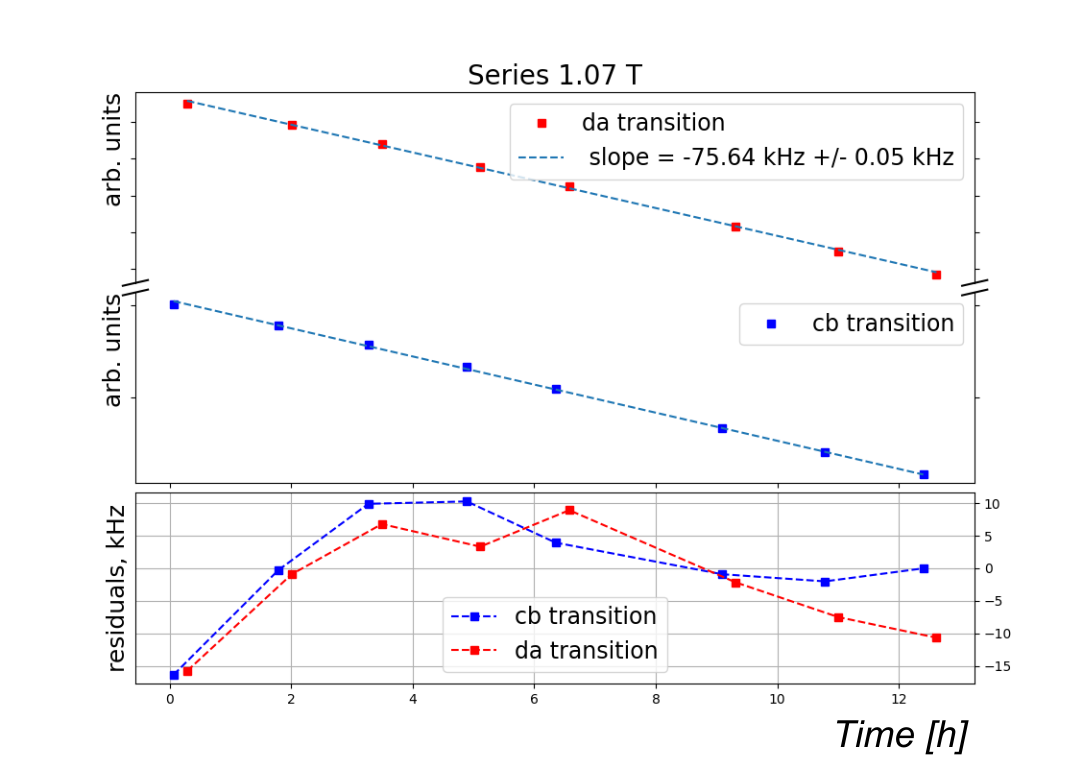
\includegraphics[width = 0.95\textwidth]{figures/chapter 4/cb_da_time_s7.png} \\
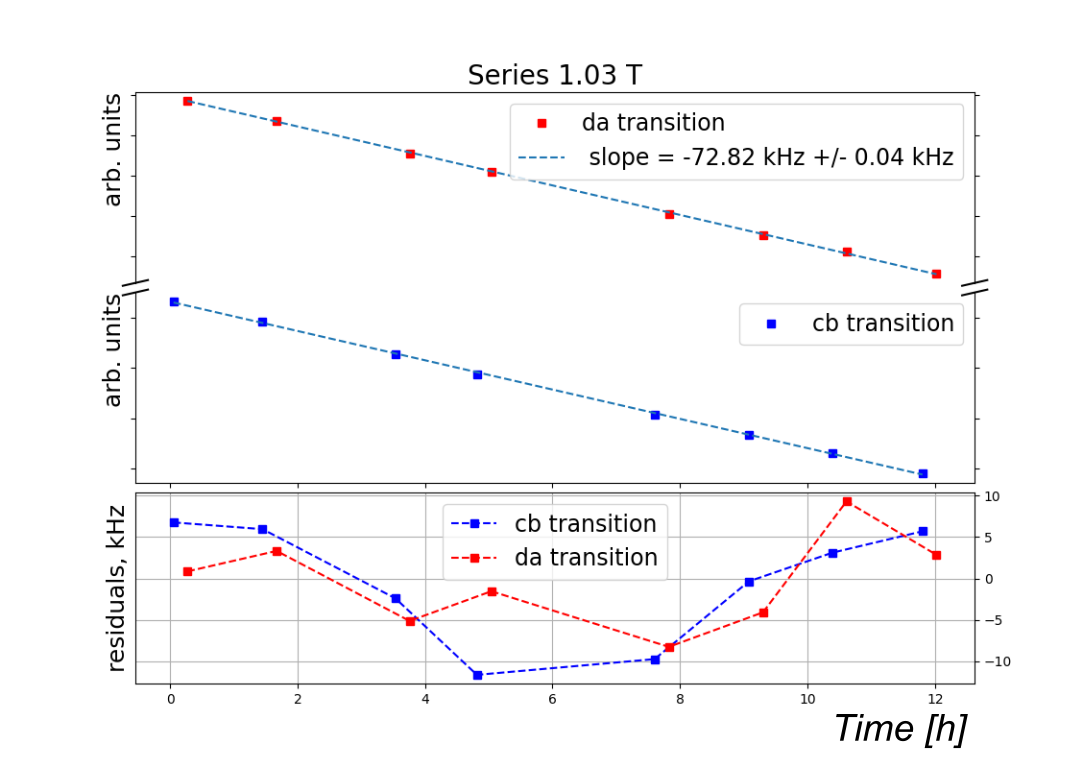
\includegraphics[width = 0.95\textwidth]{figures/chapter 4/cb_da_time_s8.png}
\caption{Frequency markers versus time for the \cb and \da transition of the high field (top) and low field (bottom) series. The blue dotted line is the extended least square fit with common slope between the two lines.}
\label{fig:FitEOLS}
\end{figure}

The plots shown in the previous figure also contain the non-normalized residuals of the linear extraction. The residuals for each individual run are also reported in Tab.~\ref{tab:resultsBdrift}, and are simply defined as: 

\begin{equation}
res_{i} = f^{i}_{cb/da}(t_{i}) - ( m_{common} * t_{i} + q \pm \frac{a_{1S}}{2h})
\end{equation}

The statistical uncertainty associated with each $f^{i}_{cb/da}$ is of order \SI{1}{\kilo \hertz}. The dispersion of the residuals around zero is not compatible with 1 standard deviation. This should not, however, be interpreted as an argument against the analysis, since the effect that certain systematics have on the position of the frequency markers has not been taken into account. In the next section, a comprehensive review of the main systematic uncertainties associated with the experimental campaign and the analysis technique is presented.

\section{Systematic Uncertainties}

This section contains a detailed explanation of each systematic uncertainty source of the ground state hyperfine splitting of the antihydrogen atom measured at ALPHA.
The systematic uncertainties have been derived mainly with a data-driven approach, which could be explained as ``what would be the result of the analysis if an alternative choice had been made?''. By looking at the discrepancies between the alternative choice and the nominal one, a systematic uncertainty is quoted. 

The measurement is affected by multiple systematic sources. Some arise from the analysis and extrapolation procedure itself (e.g., magnetic-field-drift correction, binning choices, data selection), while others are linked to properties of the data, such as lineshape variations between repetitions or between the \cb and \da transitions. Although the two transitions were equalized by tuning the applied microwave power, a residual lineshape difference remains and is included in the uncertainty budget.

As noted earlier, the key physical observable is extracted by difference: the resonance frequencies of the two transitions are not determined independently. Instead, the analysis uses fitted frequency markers—model parameters that act as proxies for resonance positions, without requiring them to be individually unbiased estimators of the true resonance frequencies. This differential strategy suppresses or cancels several systematic contributions and enables a precise measurement even in the absence of a fully realistic physical simulation of the spectra.

\subsection{The bare function \texorpdfstring{$g$}{g}}

This section contains a summary of the systematic uncertainties related to the signal model (before introducing the convolution with the asymmetric resolution function). A systematic uncertainty has been associated to the parameters controlling the signal shape, and the function choice itself.

\subsubsection{Parameters controlling the signal shape}
The shape parameters obtained from the fit to simulation, which rules the power law rise and the broadening, are used in the nominal MLE fit to extract the hyperfine splitting. However, since the simulation does not have the complete physics to fully describe the spectra, a simultaneous fit to the available high-statistics sample was performed, to benchmark the result of the simulation and to evaluate systematic uncertainty associated with the fixed parameters used in the nominal procedure.

High-statistics samples consist of runs collected with much greater stacking of atoms than the standard runs; they are used exclusively to fix certain parameters of the model and are not included in the extraction of the physics results. A total of three high-statistic repetitions were acquired: two of them for low magnetic field series (one before and one after the 8 repetitions) and one for the high field series (taken after the 8 nominal repetitions).

The high-statistics samples have been fitted with the same empirical model described above. The aim is to get an estimation from the data of the shape parameters, in particular $k$, the degree of the power law rise, in order to use that value as an alternative way in the nominal fit to extract the hyperfine splitting. The absolute difference between the nominal extracted value and the alternative analysis with $k$ is then used to quote the systematic uncertainty. Because of this, $k$ is a free parameter, shared among all the high-statistics samples. Instead of minimizing the frequency markers individually (using $f_{cb}$ and $f_{da}$ as free parameters), the fit was varied with the intention of fitting $f_{cb}$ and the splitting itself $\Delta_f$, such that the $f_{da} = f_{cb} + \Delta_f$. By doing so, it is possible to impose a common splitting between the three high-statistics repetitions too. The results of the fit are shown in Tab.~\ref{tab:highstat_floatk}, while the plot in Fig.~\ref{fig:fitwithfloatingk} shows the fit model and data.

%Minuit2Minimizer : Valid minimum - status = 0
%FVAL  = 263.837229792095229
%Edm   = 0.00086527296112601476
%Nfcn  = 11477
\begin{table}[!h]
\centering
\resizebox{\columnwidth}{!}{
\begin{tabular}{l|ccc}
\hline
\hline
\textbf{}   & \textbf{\SI{1.07}{\tesla} post}  & \textbf{\SI{1.03}{\tesla} pre}  &  \textbf{\SI{1.03}{\tesla} post}  \\
\hline 
$k$ (common)                        & \multicolumn{3}{c}{    $5.4 \pm 0.2$ }\\
$n^{(cb)}$ (common)    & \multicolumn{3}{c}{    $7.3 \pm 2.4$ }\\
$n^{(da)}$ (common) & \multicolumn{3}{c}{    $6.3 \pm 1.6$ }\\
$\sigma^{(cb)}$ (kHz)      & $17.0 \pm  0.8$  & $ 15.1 \pm 0.5  $ & $15.9 \pm 0.5$  \\
$\sigma^{(da)}$ (kHz)      & $15.8 \pm 0.7$   & $ 15.7 \pm 0.5  $ & $17.6 \pm 0.5$  \\
$\sigma^{(cb)}_{r}$ (kHz)  & $14.3 \pm  1.0$  & $ 8.9 \pm 0.6  $  & $8.7 \pm 0.6$  \\
$\sigma^{(da)}_{r}$ (kHz)  & $12.2 \pm  0.8$  & $ 11.2 \pm 0.7  $ & $9.9 \pm 0.7$  \\
$n_B^{(cb)}$               &  $ 150 \pm 22$   & $  109 \pm 20  $  &  $ 33 \pm 11$ \\
$n_B^{(da)}$               &  $ 80 \pm 16$    & $  83 \pm 21 $    &  $ 62 \pm 14$  \\
$n_S^{(cb)}$               &  $ 2271 \pm 48$  & $  2687 \pm 53  $ &  $ 2705\pm 52$ \\
$n_S^{(da)}$               &  $ 2221 \pm 48$  & $  2724 \pm 54  $ &  $ 2724\pm 52$ \\
\hline
%xZ_cb_post	  = 70.1359	 +/-  3.36124	(limited)
%xZ_cb_pre	  = 31.5012	 +/-  3.12625	(limited)
%xZ_cb_pst7	  = 47.503	 +/-  3.64418	(limited)
$\Delta f$ (kHz)           & \multicolumn{3}{c}{$ -12.7  \pm 2.8$}\\
\hline\hline
time from center of associated series (h) & $11.5$ & $-7$ & $11.2$ \\
duration of associated series (h)         & $12$ & $11.75$ & $11.75$\\
\hline
\hline
\end{tabular}
}
\caption{Model float parameters from the high-statistics samples. \label{tab:highstat_floatk}}
\end{table}

The $k$ result of the fit is 5.4, which has been used to evaluate a component of the systematic uncertainty associated with function shape variation. Since those data have been used for this task, they are not included in the main analysis, which relies only on the eight repetitions with less statistical power. 

The value of $k$ has been varied within a range whose extremes are given by the fits to the simulations and to the high-statistics samples. The nominal value $k=2$ is based on the fits to the simulations (Sec.~\ref{sec:Simulation} and Tab.~\ref{tab:resfun}). The lower extreme, $k=1$, corresponds to the lower values of $k$ obtained from the fits to the 2024 simulations ($k = 1.23 \pm 0.3$) and with the cusp resolution function, while the upper extreme, $k=5.4$, is the value obtained from the high-statistics samples. The parameter $k$ drives the extrapolation of the frequency marker: the higher its value, the further the frequency marker is from the maximum of the bare function $g$, and the larger its uncertainty, because of the longer extrapolation arm. When evaluating the systematic uncertainty associated with a larger value of $k$, this is taken into account by an additional contribution
\begin{equation}
\sigma_{syst,k} = \sqrt{\sigma^{2}_{k} - \sigma^{2}_{nominal}} \, ,
\end{equation}
where $\sigma_{k}$ and $\sigma_{nominal}$ are the statistical uncertainties of the hyperfine splitting obtained with $k = 5.4$ and with the nominal value, respectively. The results obtained with $k=1$ and $k=5.4$, together with this contribution (row \textit{max uncertainty increase}), are reported in Tab.~\ref{tab:results}, in the block \textit{bare function $g$ (parameters)}.

\begin{figure}[!htbp]
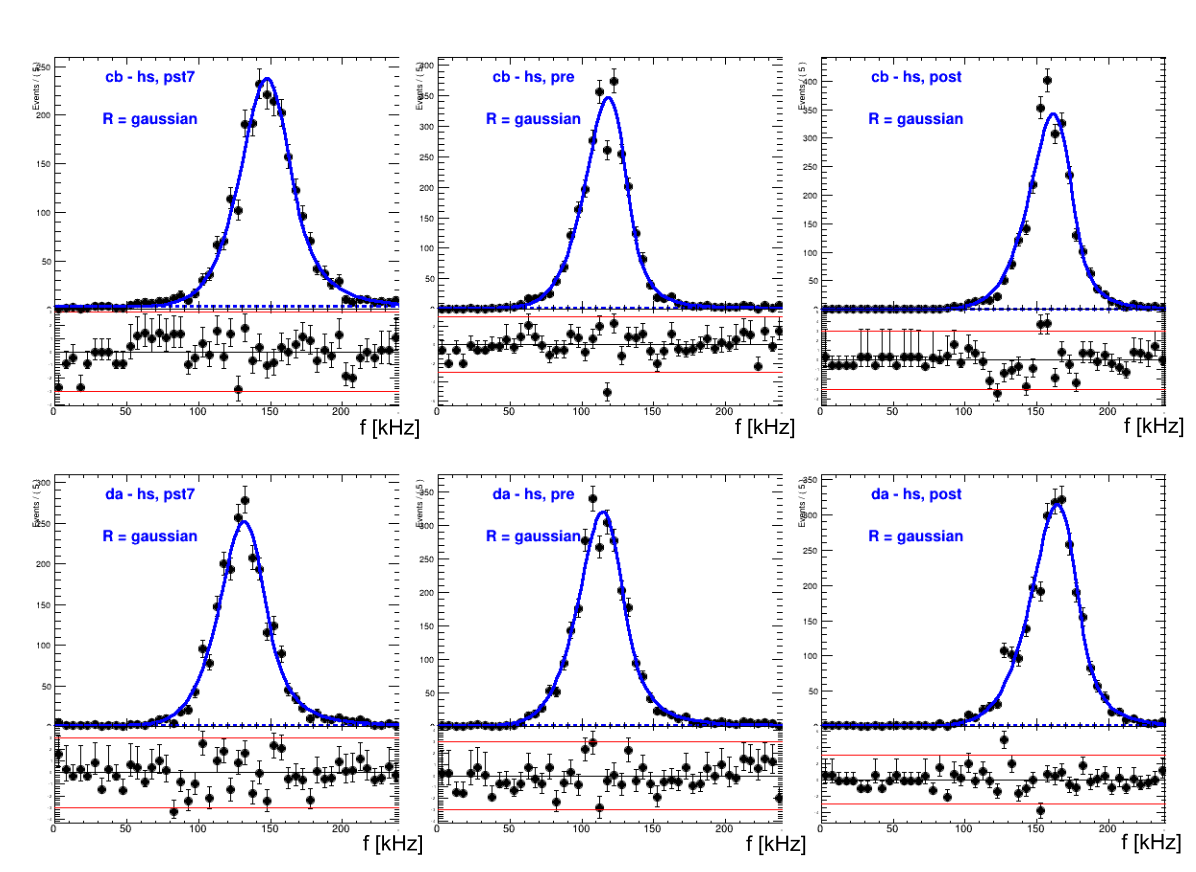
\includegraphics[width=\textwidth]{figures/chapter 4/highstat_kfloat.png}
\caption{Fit results on the high-statistics samples, with the shared $k$ parameter left free to vary in the fit, and with shared $\Delta f$, to help the convergence of the fit.}
\label{fig:fitwithfloatingk}
\end{figure}

\subsection{Alternative bare function}

An alternative function has been used to evaluate systematic uncertainty about the choice of the bare function $g$. The mathematical form of the model is:

\begin{equation}
\begin{dcases}
0 \quad \overline{x} < 0 \\
\left(\frac{\overline{x}}{\sigma}\right)^k \text{exp}\left( - \left(\frac{\overline{x}}{\sigma}\right)^{k+1} \frac{\sigma}{\sigma_r}  \frac{1}{k + 1}\right) \quad 0 \leq \overline{x} \land  \overline{x} \leq \sigma  \\
\text{exp}( \frac{\sigma}{\sigma_r} \left( \frac{k}{k+1}\right) \times \text{exp}(-\frac{\overline(x)}{\sigma_r}) \quad (\overline{x} \geq \sigma)
\end{dcases}
\end{equation}

 This model was originally developed to describe Monte Carlo simulations designed for an earlier version of the experiment, and it was deemed a suitable choice for validating the nominal empirical model. Its formulation, similarly to the nominal empirical model, was not derived rigorously from first-principles theoretical physics, but rather in a semi-empirical way.
The model considers a continuous rather than a stepped frequency ramp, and here $N_0$ is the number of trapped anti-atoms, $t_0$ is the time at which the onset condition is met, $\tau$ is the depletion rate during irradiation, and $T_{ramp}$ is the time between the onset and the peak \commento{mi sembra sia così nel modello}, and $\lambda$ controls the shape. The systematic uncertainty has been evaluated by repeating the full analysis routine with this alternative function and considering the shift in the final result compared to the nominal choice (similarly to what has been done for the majority of the systematics). The result is reported in Tab.~\ref{tab:results}, in the block \textit{bare function $g$ (choice)}.

\subsection{Frequency marker systematic uncertainty: the resolution function}

In Secs.~\ref{sec:resolutionF} and \ref{sec:Simulation} we introduced several mechanisms that broaden the observed lineshapes beyond the natural linewidth. The main contributions include magnetic-field inhomogeneity and oscillations, Doppler broadening, transit-time broadening, and microwave frequency instability. These effects are crucial because they directly affect the definition of the frequency marker.
 
A first-principles evaluation of each contribution is challenging, as it would require full knowledge of the trap dynamics, which is not available. Therefore, the approach was to vary the resolution function, both its functional form and its parameters, in order to estimate the associated systematic uncertainty on the hyperfine splitting. As a reminder, the systematic uncertainty is not linked to our ignorance of the real position of the resonance frequency given a certain transition shape. As stated before, the physical quantity is obtained through a measurement by difference, hence any point in the shape could in principle be used as a frequency marker. What really determines the accuracy of the measurement is that this frequency marker must be the same for the \cb and \da transitions. Any systematic difference in the shape of the transition directly changes the frequency marker and hence the measured splitting. In conclusion, since what matters most is the relative difference between the two transitions, this will reflect the way we have computed this systematic uncertainty.

The broadening scale, which sets the width of the resolution function, was extracted by fitting the available simulation data (see Figs.~\ref{fig:sim2023} and \ref{fig:sim2024}). Multiple spectra were simulated for different amplitudes of the microwave field in the trap cavity and analyzed using the same empirical model used for the experimental dataset. Since the onset (i.e., the transition starting point) is an input parameter of the simulation (and is placed at zero in all the simulations), it was fixed to its known value and treated as a constant. In contrast, the broadening amplitude $t_{gauss}$ and $t_{cusp}$ were left as free parameters.

\begin{sidewaysfigure}[hp]
    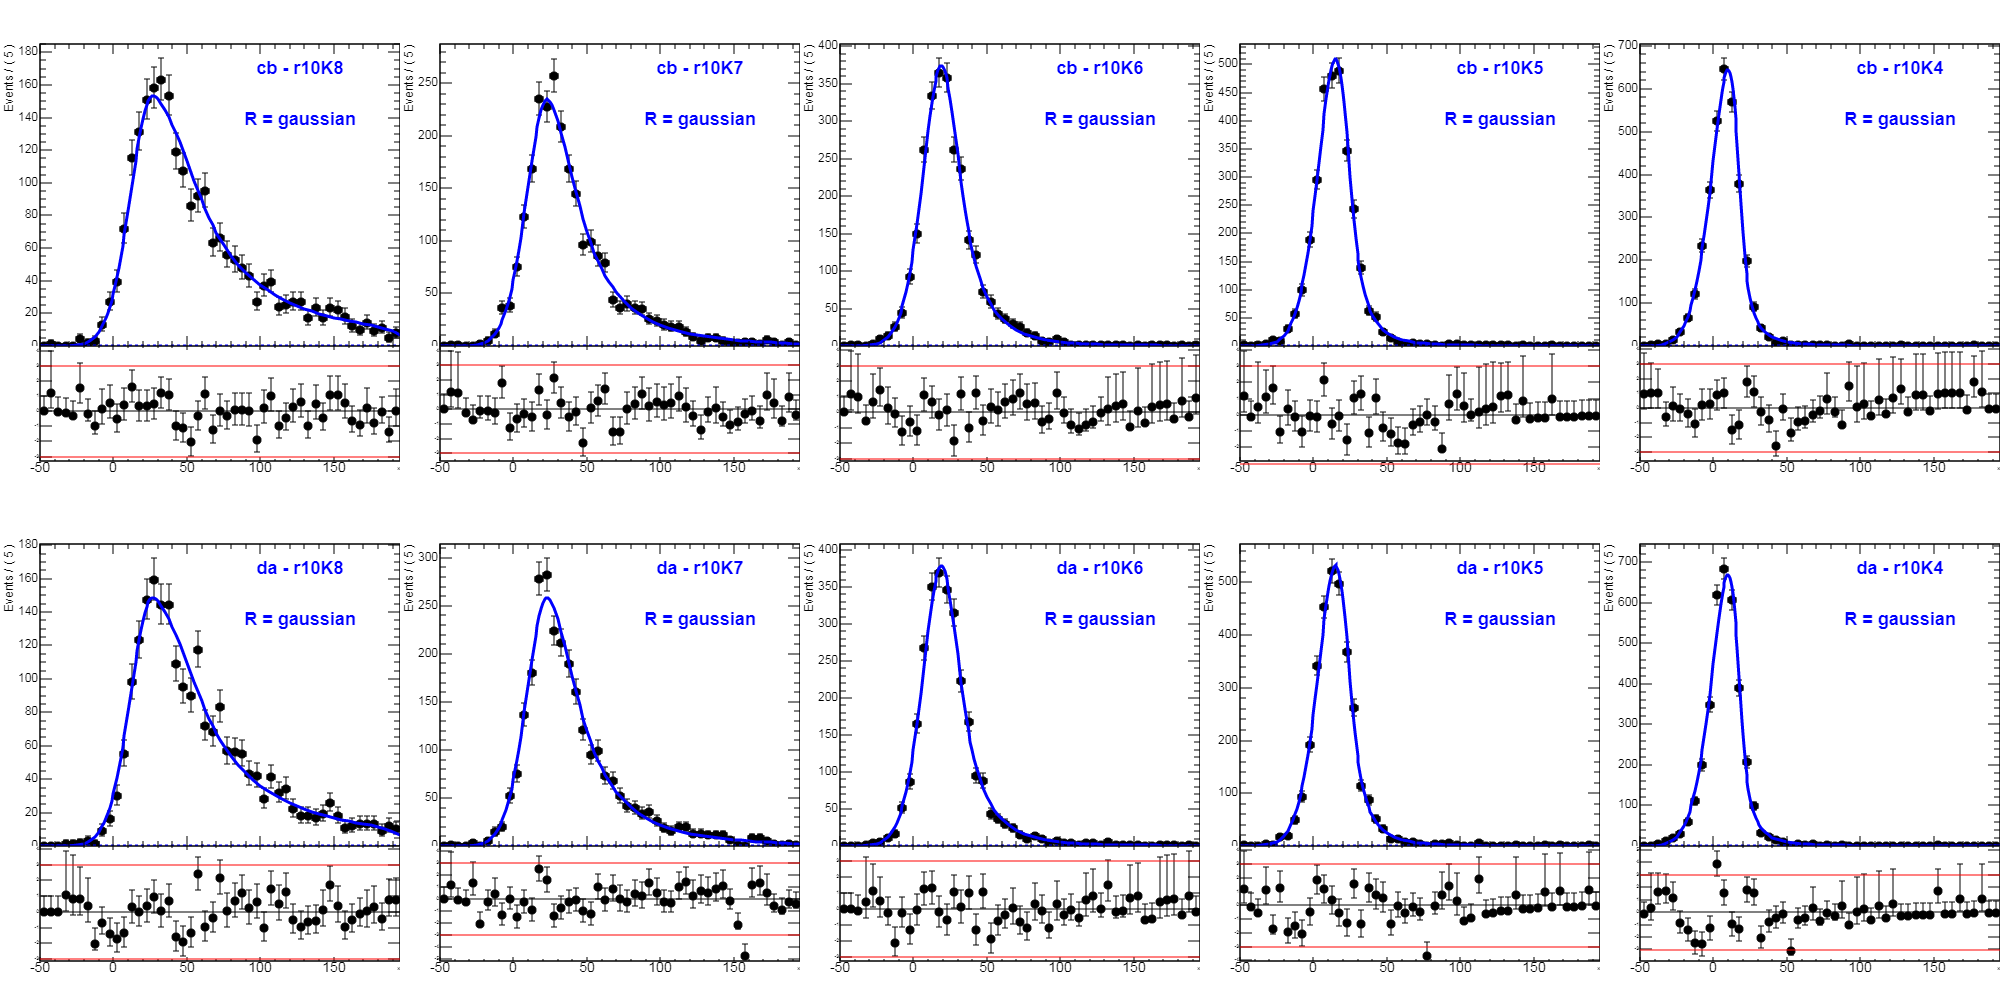
\includegraphics[width=0.65\paperwidth]{figures/chapter 4/2023_CB_gaus.png}\\
    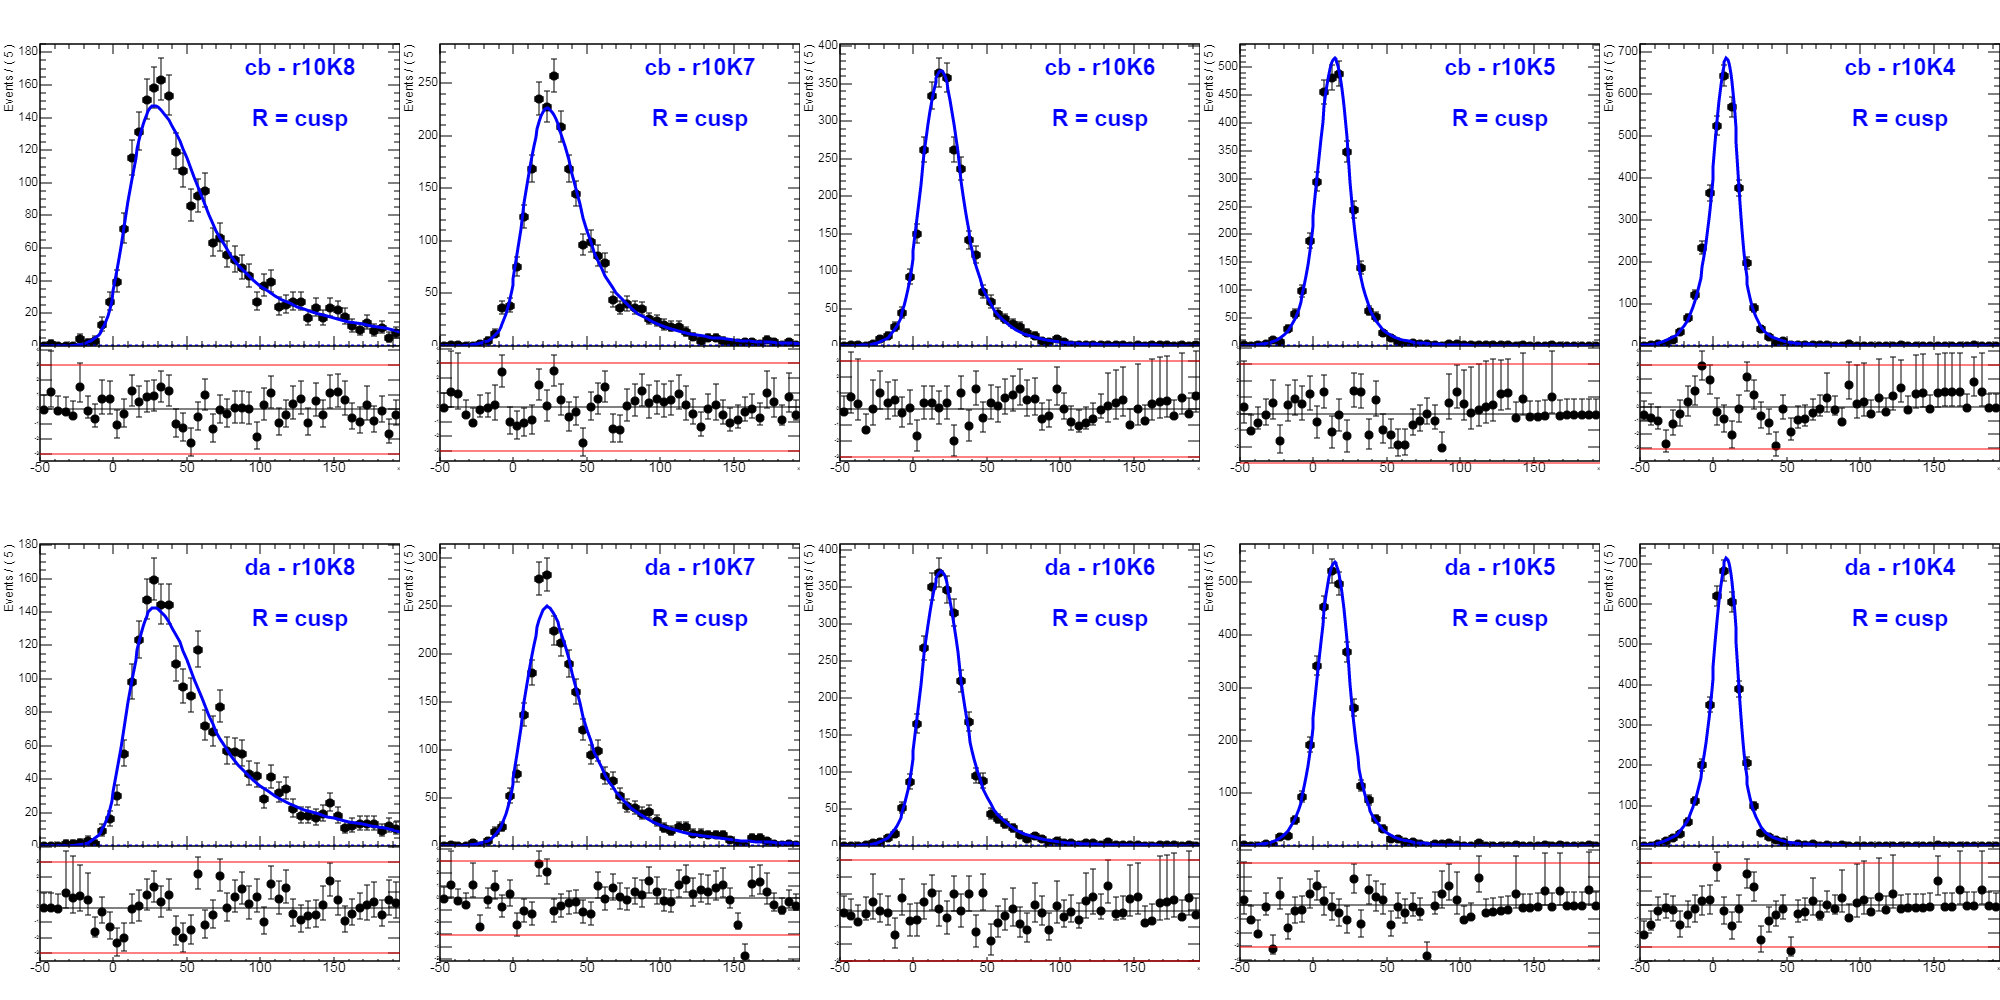
\includegraphics[width=0.65\paperwidth]{figures/chapter 4/2023_CB_cusp.png}
    \caption{Top two rows: 2023 simulations for \cb and \da transitions (the parameters are shared) with one-sided gaussian resolution function. Bottom two rows: 2023 simulations for \cb and \da transitions (the parameters are shared) with one-sided cusp function.}
    \label{fig:sim2023}
\end{sidewaysfigure}

\begin{sidewaysfigure}[hp]
    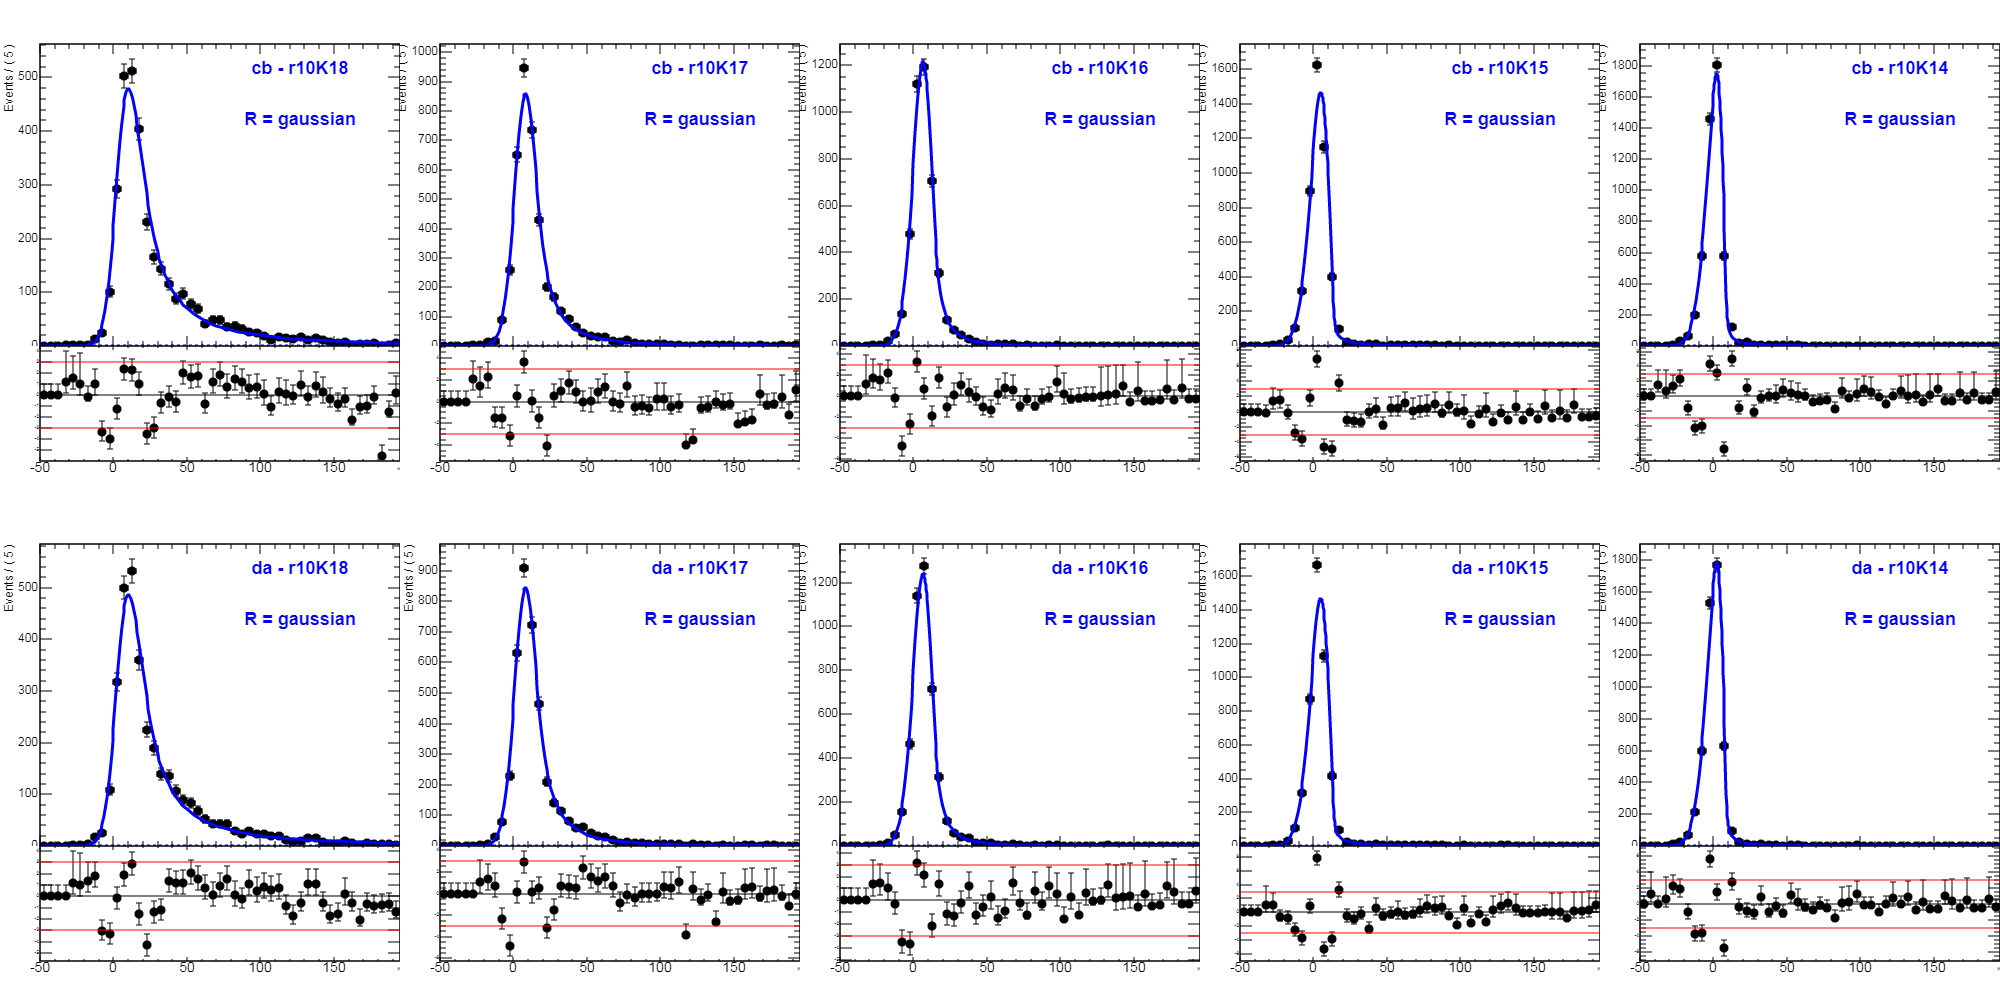
\includegraphics[width=0.65\paperwidth]{figures/chapter 4/2024_CB_gaus.png}\\
    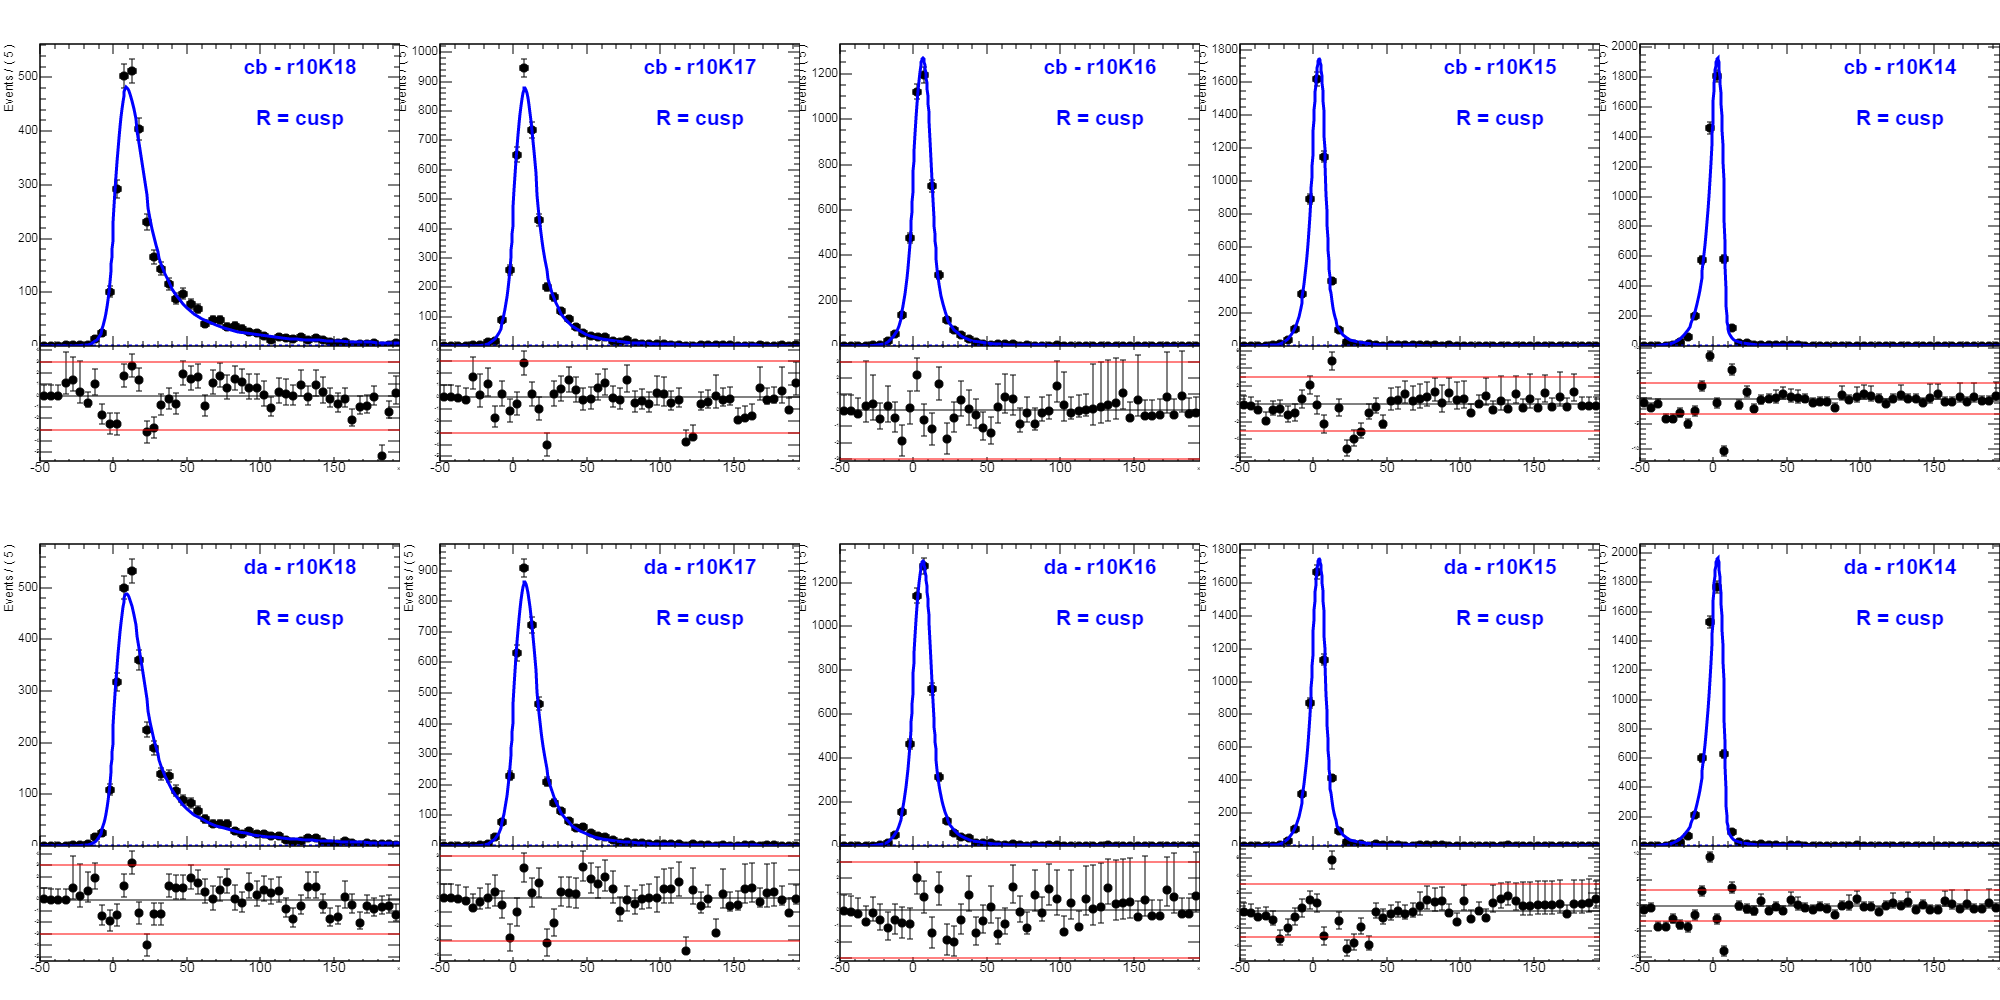
\includegraphics[width=0.65\paperwidth]{figures/chapter 4/2024_CB_cusp.png}
    \caption{Top two rows: 2024 simulations for \cb and \da transitions (the parameters are shared) with one-sided gaussian resolution function. Bottom two rows: 2024 simulations for \cb and \da transitions (the parameters are shared) with one-sided cusp function.}
    \label{fig:sim2024}
\end{sidewaysfigure}

In the nominal analysis we have used the one-sided Gaussian function as the resolution function and used the asymmetric
cusp for the model systematic. The results of the fit are summarized in Tab.~\ref{tab:resfun}. For the nominal fit to the experimental data, the broadening value was fixed to $t_{gauss} = 10 \; kHz$, as the mean value between the simulation datasets (which for simplicity are labeled as 2023 and 2024). The results indicate a reasonable range of variation of $t_{gauss}$ between the \cb and \da simulated spectra. This range of variation was used in the analysis to estimate the systematic effect related to our ignorance of the different value of broadening between the two transitions. The results are reported in Tab.~\ref{tab:results}, in the block \textit{Resolution function}: the sub-block \textit{(choice)} contains the variations of the functional form (one-sided cusp instead of one-sided Gaussian) and of the broadening common to the two transitions, while the sub-block \textit{(frequency marker)} contains mainly the variations of the broadening of one transition with respect to the other.

\begin{table}[!h]
    \centering
    \begin{tabular}{l|cc|cc}
\hline\hline
 & \multicolumn{2}{c|}{\bf Gaussian (Eq.~\ref{GaussR})} & \multicolumn{2}{c}{\bf Cusp (Eq.~\ref{CuspR})} \\ 
{\bf   Power (V/m)}  & {\bf 2023} & {\bf 2024} & {\bf 2023} & {\bf 2024}  \\
 \hline
   & \multicolumn{2}{c|}{$k$} & \multicolumn{2}{c}{$k$} \\ 
all (shared)    &  $2.47 \pm 0.2$ & $1.23 \pm 0.3$ & $1.13 \pm 0.03 $ & $0.77 \pm 0.02 $ \\
\hline  
    & \multicolumn{2}{c|}{$t_{gauss}$} & \multicolumn{2}{c}{$t_{cusp}$} \\ 
38	  & $14.8 \pm 0.2 $ & $8.9 \pm 0.1 $ & $9.1 \pm 0.2 $ & $6.3 \pm 0.1 $ \\
27	  & $14.4 \pm 0.3 $ & $8.8 \pm 0.1 $ & $8.0 \pm 0.2 $ & $5.0 \pm 0.1 $ \\
19	  & $13.9 \pm 0.3 $ & $7.7 \pm 0.1 $ & $7.2 \pm 0.2 $ & $4.6 \pm 0.1 $ \\
13.5  & $13.8 \pm 0.4 $ & $7.3 \pm 0.1 $ & $6.8 \pm 0.3 $ & $4.2 \pm 0.1 $ \\
9.5	  & $13.6 \pm 0.6 $ & $7.0 \pm 0.2 $ & $6.4 \pm 0.4 $ & $3.8 \pm 0.1 $ \\
     \hline \hline
 \end{tabular}
    \caption{Results of the fit to simulations in terms of $t_{gauss}$ for a Gaussian resolution function (see Eq.~\ref{GaussR}) and of $\tau$ for a Cusp resolution function (Eq.~\ref{CuspR}).}
    \label{tab:resfun}
\end{table}

\subsubsection{Doppler broadening} \label{sec:Doppler}

The simulations described in Sec.~\ref{sec:Simulation} do not include the Doppler effect, whose contribution to the broadening must therefore be estimated separately. Assuming a Maxwell-Boltzmann distribution for the energy of the trapped anti-atoms, and that only the component of the velocity along the direction of propagation of the microwave radiation contributes to the shift, the corresponding velocity ratio $\beta_z = v_z / c$ is normally distributed with standard deviation

\begin{equation}
\beta_z = \sqrt{\frac{k_B T}{m_{\overline{H}} c^{2}}} \, .
\end{equation}

For non-relativistic velocities the Doppler shift is $\Delta f = f - f_o = - |\beta_z| f_o$, where $f_o$ is the frequency delivered by the synthesizer. The absolute value accounts for the fact that the frequency scan is always performed from below, so that the resulting contribution to the resolution function is again one-sided, with width

\begin{equation}
\sigma_{Doppler} = \sqrt{\frac{k_B T}{m_{\overline{H}} c^{2}}} \; f_o \, .
\end{equation}

For $f_o \simeq \SI{30}{\giga \hertz}$ and an anti-atom energy distribution with a mean of $T \simeq \SI{0.36}{\kelvin}$, as measured in \cite{ALPHA:2024adiab}, this gives $\sigma_{Doppler} \simeq \SI{5}{\kilo \hertz}$; taking instead the full trap depth $T = \SI{0.5}{\kelvin}$, which is a conservative upper limit for the energy of the trapped sample, yields $\sigma_{Doppler} \simeq \SI{6}{\kilo \hertz}$.

These values are smaller than, but of the same order as, the broadening $t_{gauss} = \SI{10}{\kilo \hertz}$ extracted from the simulations and used in the nominal fit. It is therefore worth stressing that this contribution is already covered by the systematic uncertainty assigned to the resolution function: adding it in quadrature to the simulation-derived value would give an effective width of \SI{11}{\kilo \hertz} to \SI{12}{\kilo \hertz}, which lies well inside the interval $t_{gauss} \in [7.0, 13.6]\,{\rm kHz}$ explored in Tab.~\ref{tab:results}, where the induced shift of the hyperfine splitting never exceeds \SI{1.1}{\kilo \hertz}. Moreover, the estimate above should be regarded as an upper bound, since it treats each anti-atom as if it sampled the microwave field with a fixed longitudinal velocity, whereas the field in the trap is a standing wave and each atom traverses it many times within a single \SI{8}{\second} frequency step, so that the first-order Doppler contribution is largely averaged out. \commento{riassumere qui in una frase l'argomento dell'elog ALPHA/33017}

%\newpage

\subsection{Reproducibility: shape variation during the experiment} \label{sec:Reproducibility}

A possible systematic uncertainty is linked with the assumption that the shape of the spectra does not change from repetition to repetition. This assumption is used implicitly in the fit protocol, since the parameters controlling the shape of the signal model ($\sigma$, $\sigma_{r}$, and $n_{r}$) are constrained to be the same for all the \cb and \da repetitions, respectively. Hence, a dedicated study is necessary to evaluate this uncertainty.

The variation of the shape of the spectra is something expected during the measurement. There are a number of physical arguments that indicate this. At first, the energy distribution of the atom ensemble produced during the experiment can vary from repetition to repetition (although the anti-atoms are accumulated along 20 mixing cycles, and the final energy fluctuation is expected to be averaged over 20 cycles). More importantly, since the current of the main solenoid is drifting and decreasing over time, the microwave frequency must be adjusted to follow the magnetic field drift. Hence, the working point of the frequency scan changes from repetition to repetition. Following that, the microwave standing wave pattern can change, as well as the effective power delivered to the trap. Additionally, although the magnetic field profile could change during the measurement, both its on-axis profile (which can be monitored by ECR measurement) and its off-axis profile (which is unmonitored) can fluctuate due to current fluctuations in the magnets. The magnetic field profile is monitored using direct-current current transformers based on magnetometer sensors (ITZ 2000-SB FLEX ULTRASTAB from LEM International SA), and its value is used as input to PIDs that ensure the stability of each individual magnet (more details in Sec.~\ref{sec:DCCTs}).

Shape variations are expected to have a non-negligible impact on the measurement. As mentioned before, the correlation between the shape parameters and the frequency markers is strong (see Fig.~\ref{fig:CorrelationHeatMap}). Hence, shape variations from repetition to repetition are expected to consistently change the extracted value. For this reason, the experimental protocol incorporated high-statistics reference measurements, which were used to estimate the magnitude of these variations. The high-statistics sample measurement has a statistical power 5-6 times that of a single repetition. These data have been fitted independently, with the same model used in the nominal Maximum Likelihood Fit, and the results are shown in Fig.~\ref{fig:FitTOHighStats}. The parameters resulting from the fit are reported in Tab.~\ref{tab:highstatparam}.


\begin{sidewaysfigure}[hp]
\centering
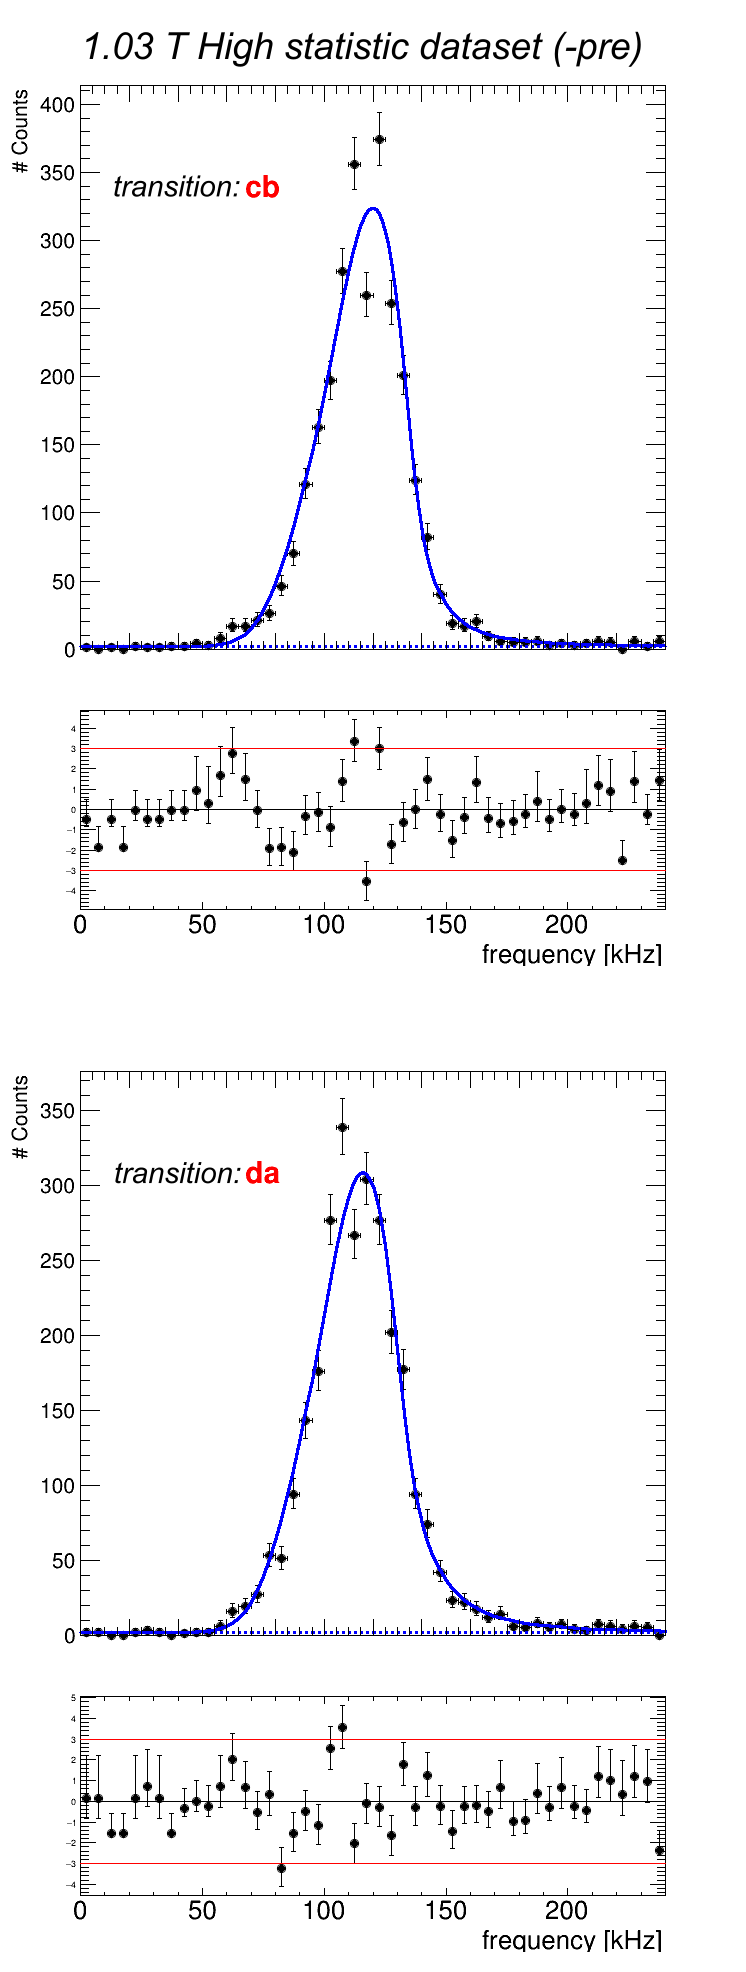
\includegraphics[width=5.2cm]{figures/chapter 4/s8_pre_v.png}  %
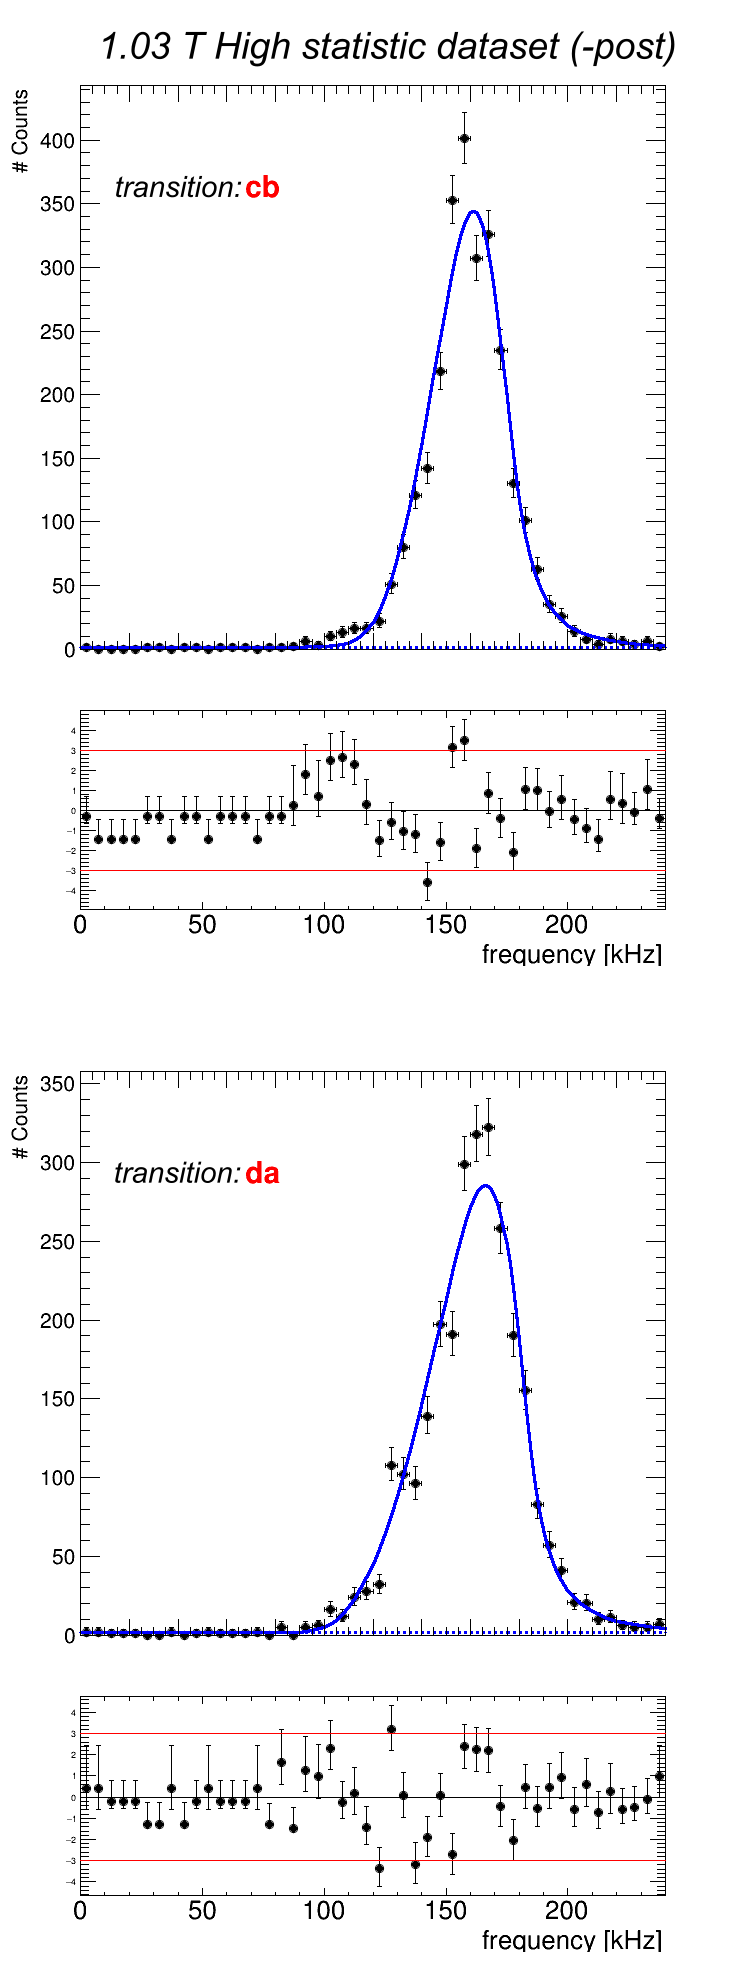
\includegraphics[width=5.2cm]{figures/chapter 4/s8_post_v.png} %
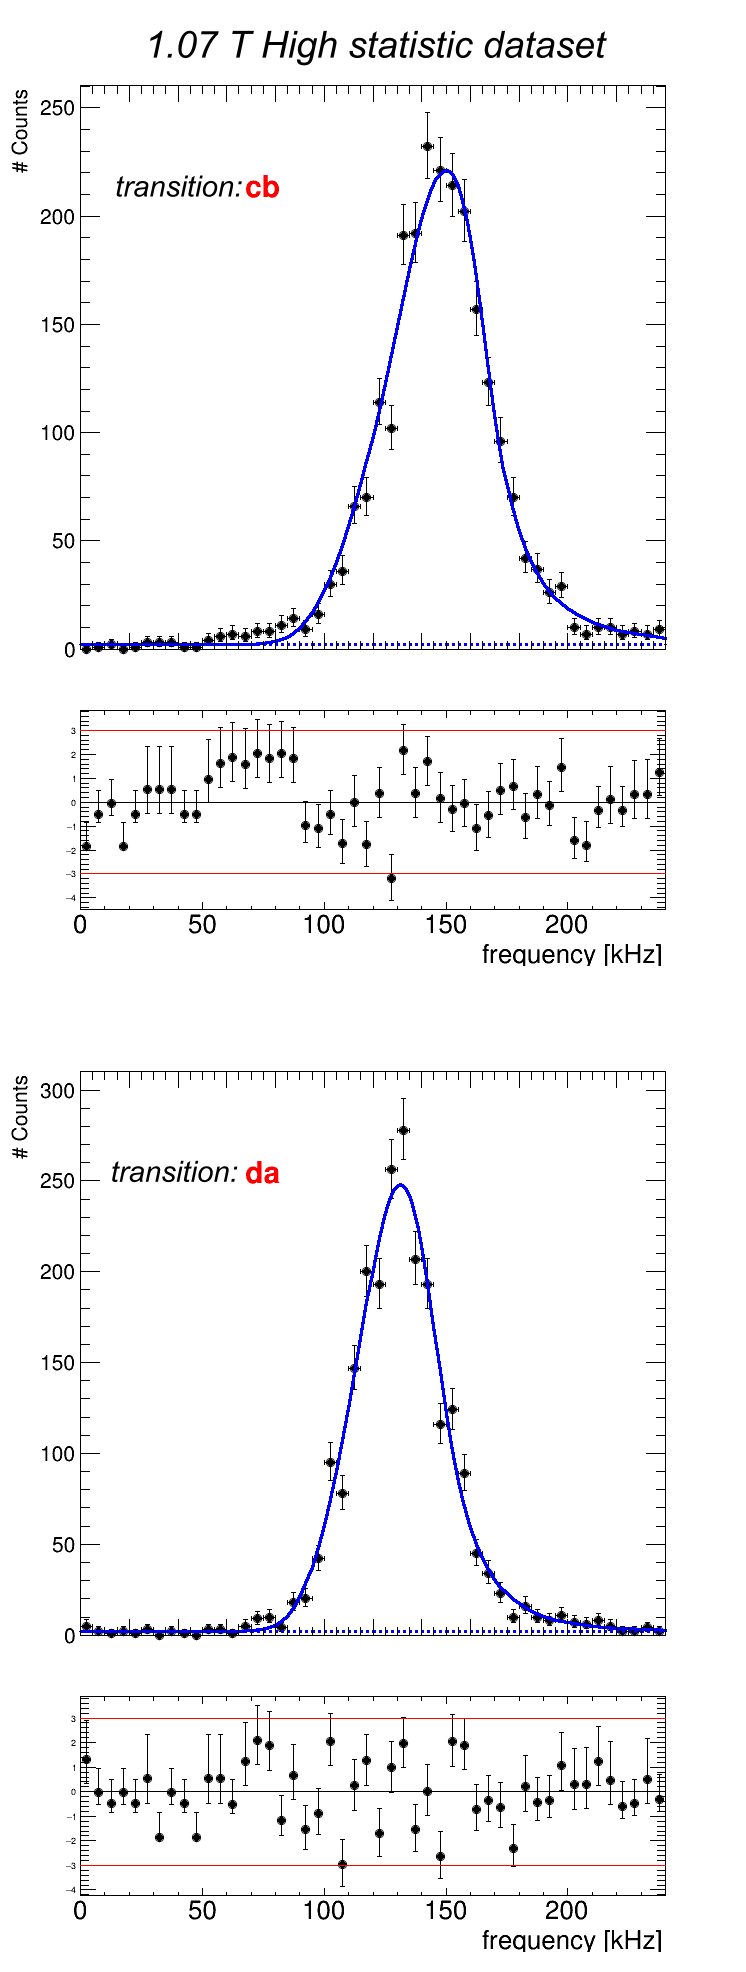
\includegraphics[width=5.2cm]{figures/chapter 4/s7_post_v.png} %
\caption{High statistic dataset for the two magnetic field configuration of the experiment. The \textit{-post} label indicated that the dataset has been acquired after the nominal 8 repetitions, the \textit{-pre} indicated that the dataset has been acquired before the nominal 8 repetitions. The fit function (blue continuous line) is the best fit result with the same model of Eq.~\ref{eq:model1}. This model constitutes a ``template'' used to estimate reproducibility uncertainty.}
\label{fig:FitTOHighStats}
\end{sidewaysfigure}

\begin{table}[!h]
\centering
\resizebox{\columnwidth}{!}{
\begin{tabular}{l|ccc}
\hline
\hline
\textbf{}  & \textbf{\SI{1.07}{\tesla} post}   & \textbf{\SI{1.03}{\tesla} pre}  &  \textbf{\SI{1.03}{\tesla} post}  \\
\hline 
$n^{(cb)}$                &  $4.3 \pm 1.7 $     & $5.1 \pm 0.9$   & $6.4 \pm 2.9$  \\
$n^{(da)}$                &  $9.8 \pm 5.6$     & $3.5 \pm 0.9$   & $3.6 \pm 1.21$  \\
$\sigma^{(cb)}_{r}$ (kHz) & $13.48 \pm  1.4$             & $7.3 \pm 0.8$   & $8.3 \pm 0.8$  \\
$\sigma^{(da)}_{r}$ (kHz) & $13.00 \pm  1.2$             & $9.0 \pm 1.0$   & $7.7 \pm 1.1$  \\
$\sigma^{(cb)}$ (kHz)     & $22.0 \pm  1.1$             & $20.3 \pm 1.0$ & $17.2 \pm 0.7$ \\
$\sigma^{(da)}$ (kHz)     & $17.1 \pm 0.9$              & $20.03 \pm 0.8$ & $24.8 \pm 0.8$ \\
$n_B^{(cb)}$              & 186 $\pm$ 25                 & 130 $\pm$ 26    &  81 $\pm$ 15   \\
$n_B^{(da)}$              & 125 $\pm$ 20                 & 86 $\pm$ 22     &  70 $\pm$ 14   \\
$n_S^{(cb)}$              & 2235 $\pm$ 51               & 2666 $\pm$ 56   &  2658 $\pm$ 53 \\
$n_S^{(da)}$              & 2175 $\pm$ 49               & 2722 $\pm$ 55   &  2716 $\pm$ 53 \\
\hline
$\Delta f$ (kHz)          & $-9.17 \pm 2.8$  &  $-8.7 \pm 2.2$  & $-20.0 \pm 2.1$ \\ %% THESE SHOULD STAY HERE. people will ask for them anyways. 
$rise^{cb}$ (kHz)         & $ 66 \pm 3$ & $ 60.8 \pm 2$ & $ 52 \pm 2$  \\
$rise^{da}$ (kHz)         & $ 51 \pm 3$ & $ 60.1 \pm 3$  & $ 74 \pm 2$  \\
\hline\hline
time from center of associated series (h) & $11.5$ & $-7$ & $11.2$ \\
duration of associated series (h) & $12$ & $11.75$ & $11.75$\\
\hline
\hline
\end{tabular}
}
\caption{Model float parameters from high statistics sample. The $\Delta f$ value (not corrected for the $B-$field drift, and blind) is shown as a cross-check.}
\label{tab:highstatparam}
\end{table}

These results can be used to evaluate the effect of shape variations on the inferred value of the hyperfine splitting. To estimate such uncertainty, only the high statistic dataset acquired after the main eight repetitions (for simplicity indicated as {\it post} distributions) have been used. Assuming a difference in shape in time, the 8 repetitions have been fitted with the model obtained from the high-statistics template, keeping all the shape parameters fixed, except the frequency markers. The full analysis procedure has been repeated and the hyperfine splitting obtained with this alternative approach has been compared with the nominal one to evaluate the systematic uncertainty. 
Since the {\it post} data were collected about $\Delta t_{post} = 12$ hours after the middle of the Physics {\it Series}, which lasted about $T_{series} = 12$ hours (see Tab.~\ref{tab:ListOfRuns}), the difference in the result has been divided by 2 (considering that the Series extends $\pm T_{series}/2 \approx \pm \Delta t_{post}/2$ around the center of the Series). This estimate resulted in \SI{2.8}{\kilo\hertz} for the high-field series (\SI{1.07}{\tesla}), \SI{7.0}{\kilo\hertz} for the low-field series (\SI{1.03}{\tesla}) and \SI{2.7}{\kilo\hertz} for their combination. The best-fit parameters for the high-statistics sample are reported in Tab.~\ref{tab:highstatparam}, while the resulting shifts of the hyperfine splitting are reported in Tab.~\ref{tab:results}, in the block \textit{Lineshape reproducibility}.

Another cross-check has been performed comparing the result of the hyperfine splitting measurement, once imposing a common rise (parameter $r$ in Eq.~\ref{eq:model1}) for the 8 repetitions (the way it is done for the measurement) and once leaving such parameter to vary across the 8 repetitions (see Fig.~\ref{fig:free_rise}) as described in Sec.~\ref{checks}. 



\subsection{Data Selection and Binning}

Uncertainties can be introduced due to the time of flight of the anti-hydrogen before annihilation and to some synchronization uncertainties. An estimate of this systematics has been evaluated by subtracting $30\,{\rm ms}$ from the time of the event, before associating the time to the frequency step. The difference with respect to the nominal case is found to be negligible. 

Binning is also a source of systematic uncertainties. All the $cb$ and $da$ scans are in fact separated by a fixed frequency difference $\delta f_{window} = 1\,420\,390\,{\rm kHz}$, which is a multiple of the $\delta_{bin} = 5\,{\rm kHz}$ frequency step. The binning chosen for the nominal analysis is aligned to the frequency step for both transitions, and the starts of the two histograms are separated by  $\delta f_{window}$. Due to the discrete nature of the scan, different choices of the binning start would have resulted in the same histograms, e.g., by starting the binning of any transition up to $\delta_{bin} -\varepsilon$ later ($\varepsilon$ is an arbitrarily small number). We assign a systematic uncertainty of $\frac{\sqrt{2}\delta_{bin}}{\sqrt{12}} = 2.0\,{\rm kHz}$ to account for this degeneracy. Both results are reported in Tab.~\ref{tab:results}, in the block \textit{Data selection and binning}.


\subsection{Short Term Upward Drift} \label{sec:ShortDrift}

The long-term linear drift is not the only effect requiring careful treatment. A short-term upward drift may also occur during the experiment. This is expected because the accumulation and stacking phase between repetitions involves changes to the beam-line magnets. Although the main solenoid magnets and mirror coil currents are not changed during this operation, the beam-line magnets must be changed, for the plasma manipulation and transport from the catching region to the atom trap. Parasitic currents could be induced in the solenoid through mutual coupling, producing a magnetic field shift distinct from the linear drift. Since the experiment is based on a \cb transition followed by a \da transition, an induced shift in the magnetic field is directly related to a systematic shift of all the \da transitions due to the Zeeman effect. Hence, a systematic shift in the splitting of the transition is expected, which is unrelated to the physical splitting.

In principle, this effect can be estimated through theoretical calculation of the parasitic currents induced from the beam-line magnets to the mirror coils and the superconducting solenoid. In practice, this approach is challenging, given the required target accuracy of this measurement. So a data driven approach was followed.

The systematic uncertainty associated with this effect has been constrained using data taken in 2023, following an experimental protocol similar to the one used for the 2024 campaign, but with specific modifications to isolate and study this effect. The protocol consisted of repeating the same measurement, a \cb and \da transition pair, with a deliberate delay introduced in the sequence between the final manipulation of the beam-line currents and the start of spectroscopy. In the first variant, the spectroscopy began \SI{32}{\second} after the last manipulation of the beam-line magnet change. In the second variant, the delay was set to \SI{352}{\second}. The delays were chosen in such a way that the \cb measurement with the second protocol coincides in time with the \da measurement of protocol 1, and the data taking consisted of alternately repeating one measurement with protocol 1 and one with protocol 2. Apart from this modification, the data-taking procedure was analogous to that employed in 2024. 6 repetitions with the first protocol and 5 repetitions with the second were taken, to correct the linear magnetic field drift and extract the transition splitting. In the following analysis, we denote $cb_{32s (352s)} ; da_{32s (352s)} $ as the frequency marker intercepts from the linear fit corresponding to the first (second) protocol. The frequency shifts induced by the short-term upward magnetic drift can then be expressed as follows:

\begin{align*}
\Delta _{cb} &= cb_{32s}  - cb_{352s} \\
\Delta _{da} &= da_{352s} - da_{32s}
\end{align*}

Three combinations of splitting can be determined from the analysis of the experimental data. The spectra were fitted using the same lineshape function as in the 2024 analysis, and the fit to the frequency markers has been performed with a slope constrained to be common to all four lines (see Fig.~\ref{fig:ShortUpwardBdrift}). Because the \cb for protocol 2 and \da for protocol 1 occur at the same time relative to the last magnet manipulation, it follows that:


\begin{figure}[!htbp]
\centering
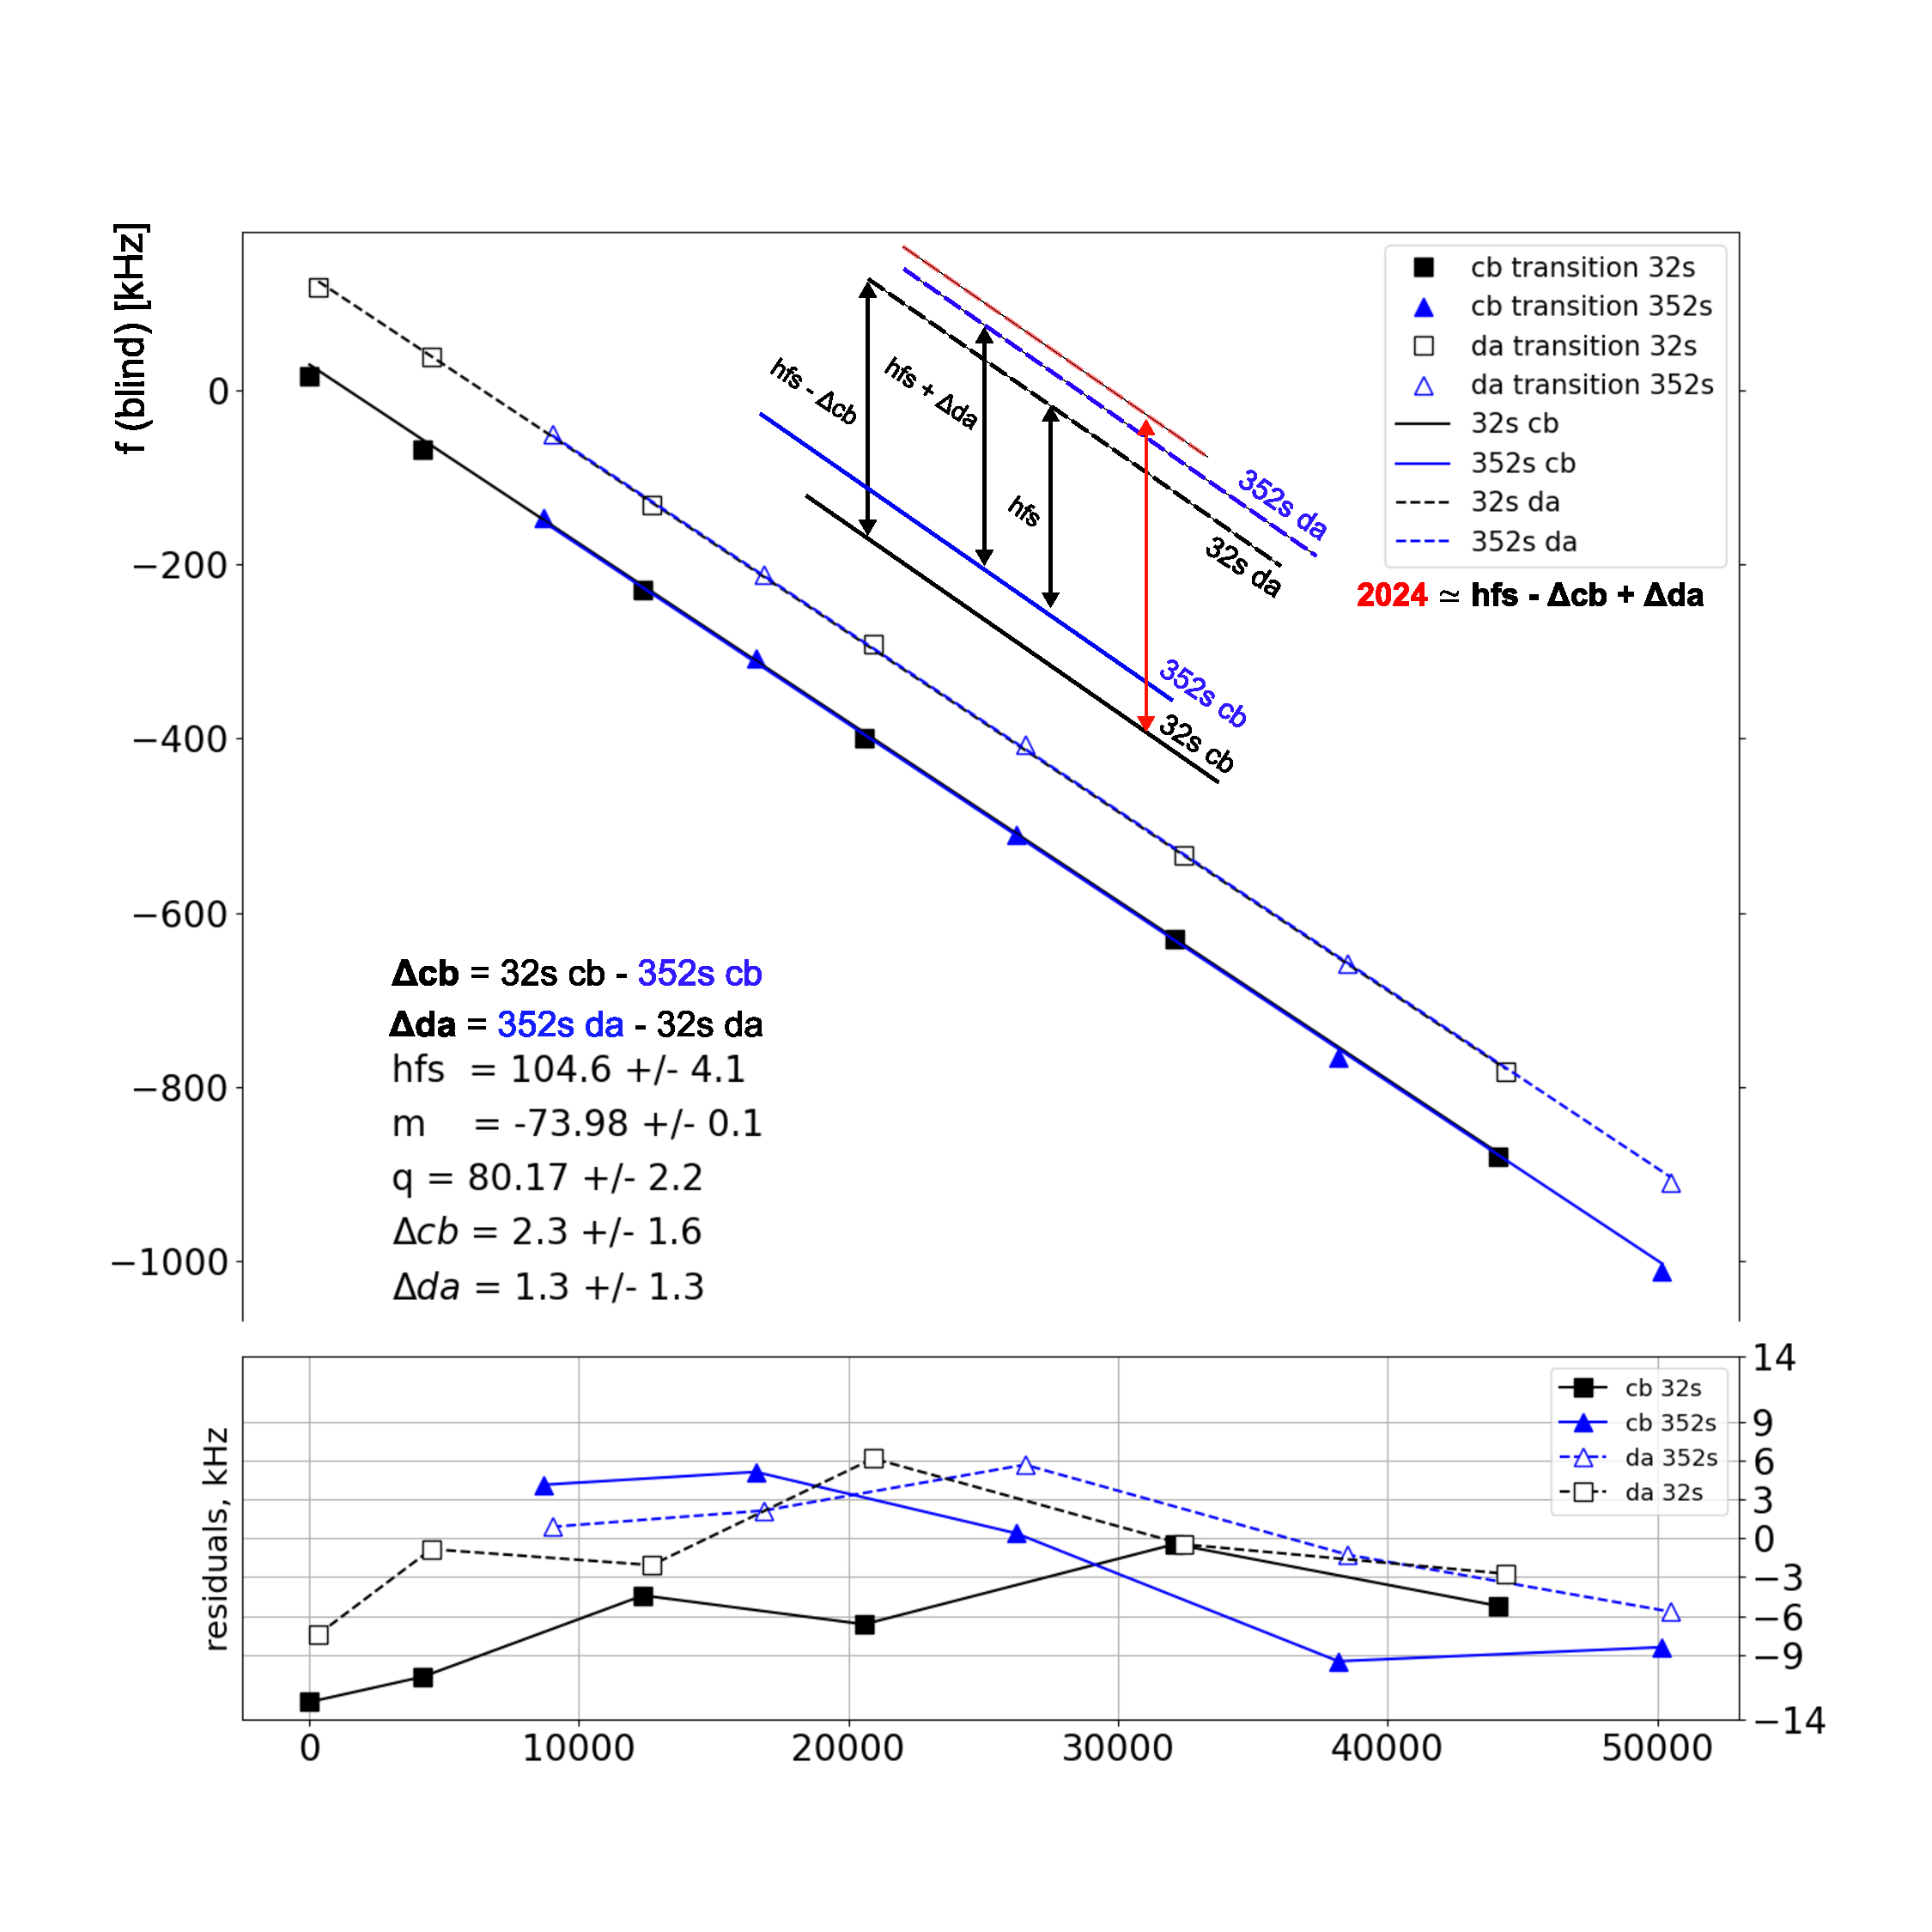
\includegraphics[width = \textwidth]{figures/chapter 4/upwardshort.pdf}
\caption{This plot shows the results from the analysis of the 2023 data. This analysis has been used to constrain magnetic upward drift induced from beam-line magnet manipulation during antihydrogen stacking phase. The change of the beam-line magnets during stacking can induce parasitic currents on Mirror and Solenoid magnets, causing a small magnetic upward drift. Since the \da transition always follows the \cb transition, this effect can generate a systematic shift in the frequency that changes the value of the splitting. This shift has been constrained using 2023 data that were collected with two protocols. In the first protocol there are \SI{32}{\second} between the last manipulation of the beam-line magnets and the start of the microwave measurement. In the second protocol the time interval is increased to \SI{352}{\second}. With this setup, the \cb transition with the \SI{352}{\second} delay starts at the same time, with respect to the beam-line magnet manipulation, of the \da transition with the \SI{32}{\second} delay. The frequency markers shown are the result of the analysis on Pass Cuts data.}
\label{fig:ShortUpwardBdrift}
\end{figure}


\begin{equation*}
a_{1S}/h = da_{32s} - cb_{352s}
\end{equation*}

The other two quantities of interest are:

\begin{align*}
da_{352s} - cb_{352s} &= da_{32s} + \Delta_{da} - cb_{352s} = a_{1S}/h + \Delta_{da}  \\
da_{32s}  - cb_{32s}  &= da_{32s} - \Delta_{cb} - cb_{352s} = a_{1S}/h - \Delta_{cb}
\end{align*}

The linear fit was performed with the same minimization technique (extended least-square), with a common slope $m$, the hyperfine splitting $a_{1S}/h$, common offset $q$ and shifts $\Delta_{cb}$ and $\Delta_{da}$ as free parameters. The best fit values have been reported in Fig.~\ref{fig:ShortUpwardBdrift}. 
The 2024 data taking had the \cb measurement starting \SI{32}{\second} after the beam-line manipulation, and the \da transition was measured after \SI{512}{\second} + \SI{300}{\second} of wait. So the overall shift can be approximated as:

\begin{equation}
da_{2024} - cb_{2024} \simeq da_{352s} - cb_{32s} = a_{1S}/h - \Delta_{cb} + \Delta_{da}
\end{equation}

From this analysis, the systematic shift due to the short-term upward magnetic shift was estimated as $\sigma_{shift} = |  \Delta_{da} - \Delta_{cb}| = 1 \; kHz$. This value has been added in quadrature as a systematic uncertainty to the overall error budget of the measurement, and is reported in Tab.~\ref{tab:results}, in the block \textit{B-drift (short time scale drift)}.


\subsection{Magnetic decay over time} \label{sec:decaySystematic}

As mentioned in the experimental protocol (Sec.~\ref{Protocol-of-experiment}), the decay of the magnetic field has to be corrected in the analysis to extract the hyperfine splitting. The magnetic field drift can be characterized with ECR measurement and with spectroscopy itself. In the current analysis, no ECR measurements were used to account for the drift, and the magnetic field has been introduced as a parameter in the common linear fit. Hence, an assumption of a linear decay has been used in the main analysis, and a systematic uncertainty must be assigned to account for this particular choice.

A first alternative is the so-called ``split'' method, which was used in a previous version of the analysis and provides an estimate of the hyperfine splitting for each individual repetition. Instead of the common fit, two separate linear fits are performed to the \cb and to the \da frequency markers, and the average of the two slopes, $m_{split} = (m_{cb} + m_{da})/2$, is used to correct the difference between the two markers of each repetition for the field drift that occurs during the interval $\Delta t = \SI{812.4}{\second}$ between the two scans:

\begin{equation}
\Delta f^{(i)}_{corr} = f_{da}^{(i)}(t_i + \Delta t) - m_{split} \Delta t - f_{cb}^{(i)}(t_i) \, .
\end{equation}

With slopes between about $-72$ and \SI{-76}{\kilo\hertz\per\hour}, the correction amounts to roughly \SI{17}{\kilo\hertz}. The hyperfine splitting is then obtained from the average of the eight $\Delta f^{(i)}_{corr}$ of each series, to which the separation $\delta f_{window}$ between the two scans is added. The results of the ``split'' method differ from the nominal ones by \SI{-2.3}{\kilo\hertz} and \SI{+0.5}{\kilo\hertz} for the high-field and low-field series, respectively, as reported in Tab.~\ref{tab:results}, in the block \textit{B-drift (fit procedure)}. The origin of this discrepancy has been attributed to the fact that the ``split'' method neglects the off-diagonal blocks of the covariance matrix of Tab.~\ref{tab:cov_matrix}, i.e.\ the correlation between the differences $\Delta f^{(i)}$ and the \cb markers, which is instead taken into account by the common GLS fit.

A Gaussian process regression (\textit{GPR}) technique has been employed as a second alternative method to correct for the magnetic field drift over time. Instead of testing different decay models, Gaussian process regression uses non-parametric supervised learning methods to solve regression problems. This method allows for an alternative estimate of the hyperfine splitting without relying on the assumption of a linear decay of the field. This technique has been applied to the average of the frequency markers:

\begin{equation}
\overline{f}^{i} = \dfrac{f^{i}_{cb} + f^{i}_{da}}{2}
\end{equation}

 The $\Delta_{f}^{i} = f_{da}^{i} - f_{cb}^{i}$ have been corrected for the magnetic field drift individually (by estimating the frequency shift from the time interval between the \cb and \da, i.e.\ \SI{812.4}{\second}, and considering each individual local magnetic drift). The result of the GPR interpolation is shown in Fig.~\ref{fig:GPR}.

\begin{figure}[!htbp]
    \centering
    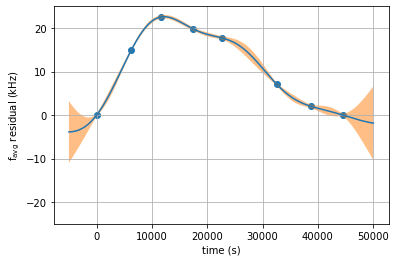
\includegraphics[width=0.49\linewidth]{figures/chapter 4/s7_residual_gpr0.2.png} 
    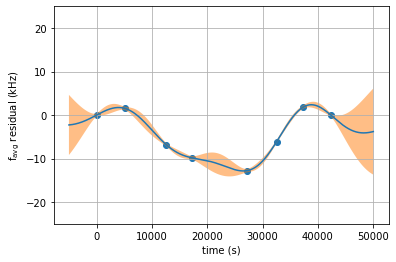
\includegraphics[width=0.49\linewidth]{figures/chapter 4/s8_residual_gpr0.2.png} \\
    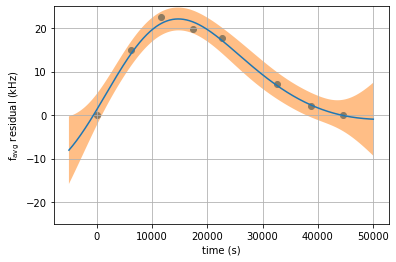
\includegraphics[width=0.49\linewidth]{figures/chapter 4/s7_residual_gpr2.0.png} 
    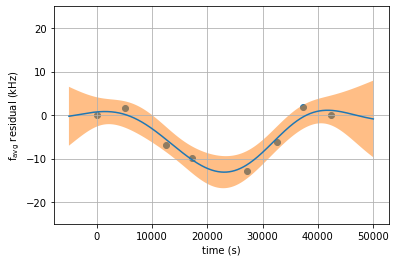
\includegraphics[width=0.49\linewidth]{figures/chapter 4/s8_residual_gpr2.0.png} 
    \caption{Interpolation of the $cb$ frequency markers (points) with Gaussian Process Regression for the high-field (left) and low-field (right) series. The linear trend is removed before interpolation 
    (detrending is such that the ordinates of the first and last points are zero). The abscissa is the time of the repetition in seconds and the ordinate is the residual w.r.t. the linear trend of the frequency markers, in kHz. The band represents the $95\%$ confidence interval.
    Top and bottom figures are obtained with different settings for the input noise, without significant changes in the estimate of the systematic uncertainty. The top plots correspond to the settings used for the estimate in Tab.~\ref{tab:syst}.}
    \label{fig:GPR}
\end{figure}

Since the GPR correction is applied to the individual differences, the result is compared with the ``split'' method with linear correction. The differences between the two are \SI{-0.3}{ \kilo \hertz} and \SI{-0.1}{\kilo \hertz} for the high B-field and low B-field series, as reported in Tab.~\ref{tab:results}, in the block \textit{B-drift (long time scale linearity)}.

\subsection{DCCT Traces and Magnetic Field Fluctuation} \label{sec:DCCTs}

The magnets employed to design the microwave flat magnetic field for the measurement are supplied with hundreds of amperes, and are handled and monitored with direct-current current transformers based on closed-loop fluxgate magnetometer sensors (DCCT). The current flowing in each magnet is constantly measured by an analog-to-digital converter (NI-9239 cRIO) that digitizes the DCCT signal output, and it is used in PID control of the magnet power supply for stabilization within a few mA. In the context of the analysis, the DCCTs current traces have been analyzed to verify how stable the currents are versus time. 

\begin{figure}[hbtp]
\centering
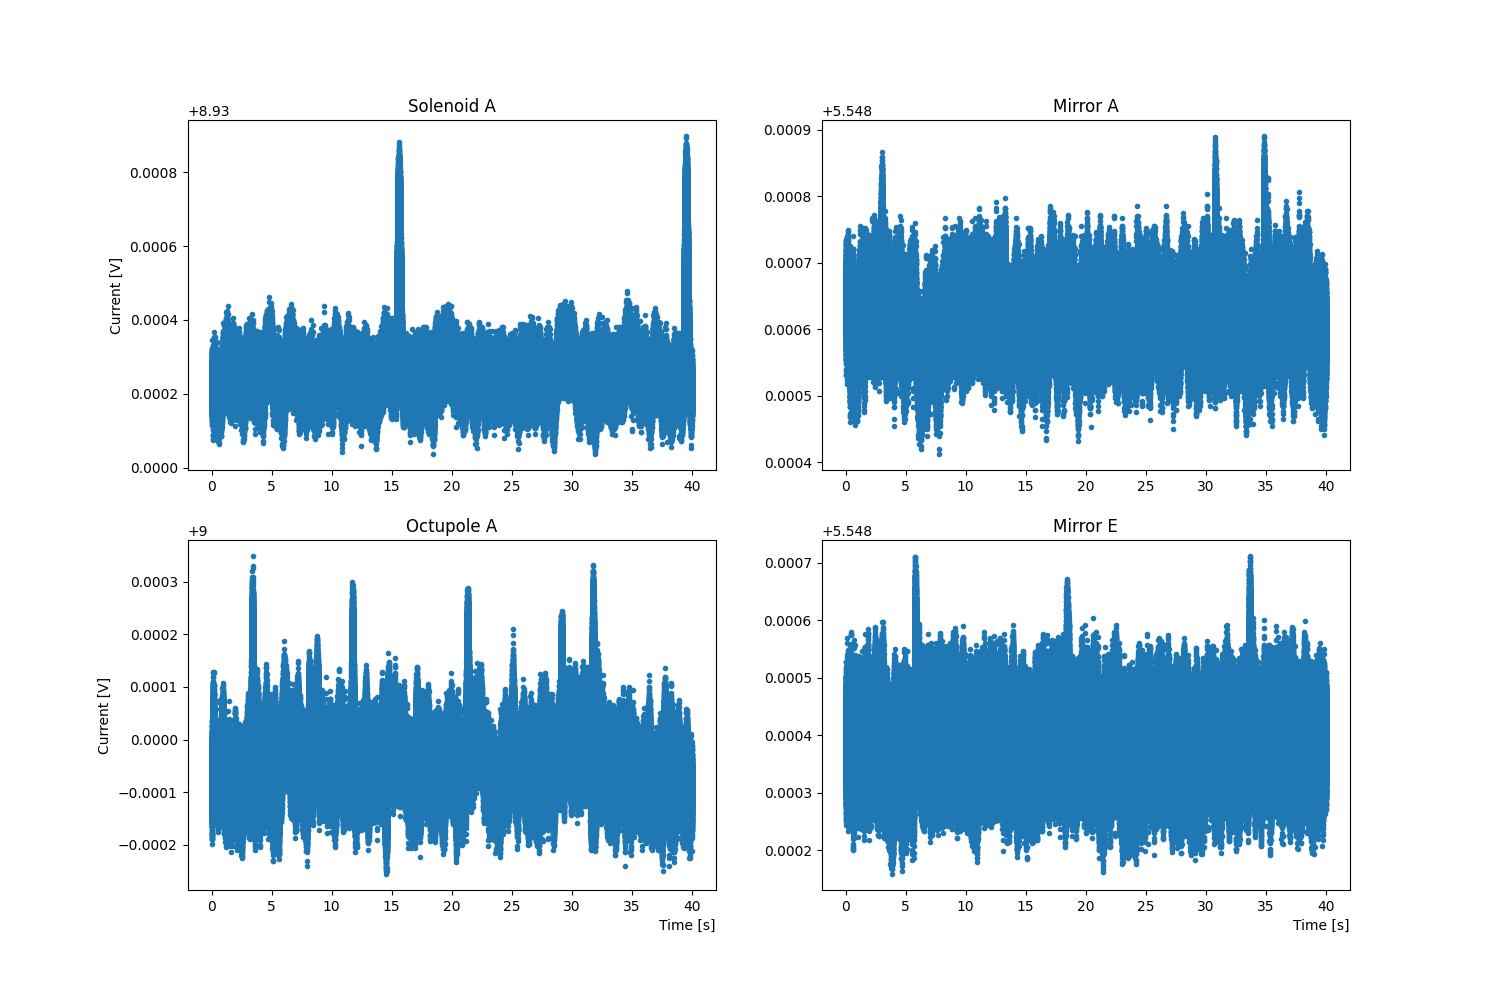
\includegraphics[width = \textwidth]{figures/chapter 4/Example_of_DCCTs_traces.png}
\caption{Example of DCCTs traces for a total of 40 second of acquisition. The units on the y-axis are Volts, since the DCCT provides a $\pm 10 $ V output. The traces have been converted into Ampere units and the amplitude of the glitches has been used to study possible discrepancies on the measurement induced by changes in the magnetic field minimum.}
\label{fig:DCCTsTraces}
\end{figure}

As evident in Fig.~\ref{fig:DCCTsTraces}, the DCCT traces for a selection of magnets show that there are glitches in the magnet currents occurring on a \SI{10}{\kilo \hertz} scale. These glitches could potentially influence the magnetic field profile along the axis, which can result in a temporary (fast) change in the resonance frequency of the atoms. Although the duration of the observed glitches for all the magnets has been confirmed to be short (less than \SI{0.1}{\second}), their amplitudes, when translated into \SI{}{\kilo \hertz} units, were non-negligible (of the order of \SI{10}{\kilo \hertz}).

Such an effect can potentially displace and anticipate some of the annihilations that would occur later during the microwave scan. Hence, an ad-hoc simulation study was performed to estimate how much such displacement occurring with a certain rate would affect the hyperfine splitting measurement. 

The simulation was performed by creating pseudo-data from the real datasets. Glitches similar to the ones observed in Fig.~\ref{fig:DCCTsTraces} were simulated with a time rate of \SI{10}{\hertz}. Each time a glitch happens, it is chosen randomly from a list containing all the glitches observed during the \SI{40}{\second} of DCCT traces measured. Each glitch was approximated as a step function, with a duration fixed to be equal to the interval over which the glitch goes from $10$ percent (before peak) to $10$ percent (after peak), and an amplitude equal to the observed peak. By considering the peak, we overestimate the displacement of the annihilations. 

The simulation considers the displacement to be asymmetrical. This means that negative current glitches (where the magnetic field decreases) anticipate annihilations happening later on in the spectra, while positive glitches delay some of the annihilations to the next bin. With this simulation mechanism, pseudo-data were generated and fitted with the same nominal protocol used in the analysis. The simulation consisted of 40 pseudo-experiments, and the standard deviation of the results was used to estimate the effect on the splitting. The standard deviation of the results obtained for both series is \SI{0.7}{\kilo \hertz}, which is small compared to other systematic uncertainties. Besides this, further consideration indicates that assuming a 100 \% conversion from current to frequency displacement is a generous overestimation. In fact, because of the coupling between different magnets, the mutual induction contributes to mitigating the effect on the magnetic field profile. This computed value is to be considered as a cross-check that shows that, if such a mechanism is present, its influence on the measurement is small; hence it was not considered in the final estimation of the systematic uncertainty.

\subsection{Error Budget Table} \label{sec:ErrorBudgetSec}

This section contains the error budget table, which contains all the alternative results of the analysis by the different methodologies that have been considered for systematic studies. The first row, indicated with \textit{Nominal,(``common fit'' linear GLS)}, represents the final analysis result with the nominal parameters and methodology. The reported result is blinded, and the frequency separation used during the experiment (the separation between the \cb and \da microwave sweeps), which is equal to \SI{1420390}{\kilo \hertz}, is not added to the final result. All the remaining rows represent different analysis methodologies that have been considered to estimate the various systematic uncertainties. All results are blinded using the same blinding value, so that they all share a common offset and can therefore be directly compared; they are grouped into separate sections, according to the specific effect each alternative approach is intended to address. The systematic uncertainty is estimated from the difference between the \textit{Nominal} result and the alternative approach. This difference has been reported for each alternative approach in a separate column indicated with \textbf{$\Delta$}. For each sub-group, the maximum difference has been taken as the nominal systematic uncertainty, and is reported in summary Tab.~\ref{tab:syst}. The last column contains the combination of the two series, and the results are obtained by the weighted mean of the results of the two series using the statistical error as weight.

\begin{table}[!h]																			
\small 
\centering
\scalebox{0.8}{
\begin{tabular}{l||r|l||r|l||r|l}																			
%\hline
%\multicolumn{7}{c}{GLS COMBINED LINEAR FIT} \\
\hline								\hline		
\textbf{Configuration} & \multicolumn{2}{c||}{\textbf{High field (kHz)}} & \multicolumn{2}{c||}{\textbf{Low Field (kHz)}} & \multicolumn{2}{c}{\textbf{Combination}} \\																			
	& $	a^{blind}_{1S}/h	\pm	\sigma$ & $	\bf{\Delta}$ & $ a^{blind}_{1S}/h \pm	\sigma$ & $\bf{\Delta}$ & $ a^{blind}_{1S}/h \pm	\sigma$ & $\bf{\Delta}$ \\
\hline																			
\hline												 
{\it Nominal (``common fit'' linear GLS)} & & & & & & \\							
$k=2$, $t_{gauss}^{cb}=10$, $t_{gauss}^{da}=10$  & {\bf \textcolor{blue}{ 10.83 $\pm$ 1.7  }}  & $ - $  & { \bf \textcolor{blue}{8.98 $\pm$ 1.5}}  & $ - $ & {\bf \textcolor{blue}{9.79 $\pm$ 1.1} }  & $ - $\\
\hline 
\hline 
{\it Lineshape reproducibility} & & & & & & \\
Nominal with g from post	                     & $ 16.48 \pm 0.4 $ & $ (5.65)	 $    & $-4.98 \pm 0.4 $ & $ (-13.96) $       & $4.41 \pm 0.3$ & $-5.38$ \\
{\it $\Delta$ is divided by 2 (see text)}        &                   & $ {\bf 2.8 } $ &                  & ${\bf -7.0}$     &                & ${\bf -2.7}$ \\
\hline 
\hline
{\it bare function $g$ (choice)} & & & & & & \\
Alt. bare function, $k=2$, $t_{cusp}=6$	          & $ 11.28 \pm 1.4$ & ${\bf 0.5}$    & $9.65	\pm 0.4$ & ${\bf 0.7}$      &  $10.36 \pm 0.4$& ${\bf 0.6}$ \\
\hline
{\it (parameters)} & & & & & & \\
$k=1$& $8.32  \pm 1.0 $       & $ {\bf -2.5}$     & $9.31 \pm 0.8 $    & $ 0.3 $     & $8.88 \pm 0.6$ & ${\bf -0.9}$ \\
$k=5.4$ & $10.70 \pm 3.8 $    & $ -0.1$           & $10.01 \pm 3.2 $   & {\bf  1.0 } & $10.31 \pm 2.4$& $0.5$  \\
\nullo{$k=5.4$, $t_{gauss}^{cb}=10$, $t_{gauss}^{da}=10$}	max uncertainty increase & ($\sqrt{3.8^{2}-1.7^{2}})$ & {\bf 3.4 } & ($\sqrt{3.2^{2}-1.5^{2}})$ & {\bf 3.0} & ($\sqrt{2.4^{2} - 1.1^{2}}$) & {\bf 2.1}\\
\hline
\hline 
{\it Resolution function} & & & & & & \\
{\it (choice)} & & & & & & \\
$t_{cusp}^{cb}=t_{cusp}^{da}=5.1$	    & $11.15 \pm 1.7 $ & ${\bf 0.3 } $ & $8.99 \pm 1.4 $ & $ 0.0$       & $ 9.94 \pm 1.1$ & $0.2$ \\
$t_{gauss}^{cb}=t_{gauss}^{da}=13.6$	& $11.00 \pm 1.9 $ & $ 0.2 $       & $9.22 \pm 1.6 $ & $ 0.2 $      & $10.00 \pm 1.2$ & $0.2$ \\
$t_{gauss}^{cb}=t_{gauss}^{da}=7.0$	    & $10.9  \pm 1.6 $ & $ 0.1 $       & $9.62 \pm 1.4 $ & $ {\bf 0.6}$ & $9.83  \pm 1.1$ & ${\bf 1.1}$  \\
\hline
{\it (frequency marker)} & & & & & & \\
$t_{gauss}^{cb}=10$, $t_{gauss}^{da}=8$	 & $7.64 \pm 1.7 $   & $ -3.2$      & $5.87 \pm 1.5 $   & $ -3.1$       & $6.64 \pm 1.1$ & $-3.2$ \\
$t_{gauss}^{cb}=10$, $t_{gauss}^{da}=12$ & $14.34 \pm 1.8 $  & ${\bf 3.5 }$ & $12.35 \pm 1.5 $  & $ 3.4$        & $13.22 \pm 1.2$& ${\bf 3.4}$  \\
$t_{gauss}^{cb}=8$, $t_{gauss}^{da}=10$	 & $13.75 \pm 1.7 $  & $ 2.9 $      & $12.45 \pm 1.4 $  & $ {\bf 3.5 }$ & $13.02 \pm 1.1$& $3.2$  \\
$t_{gauss}^{cb}=12$, $t_{gauss}^{da}=10$ & $7.43 \pm 1.8 $   & $ -3.4 $     & $5.74 \pm 1.5 $   & $ -3.2$       & $6.48 \pm 1.2$ & $-3.3$ \\
$t_{gauss}^{cb}=t_{gauss}^{da}=0$        & $11.97 \pm 1.6 $  & $ 1.1$       & $9.89 \pm 1.3 $   & $0.9 $        & $10.80 \pm 1.0$& $1.0$   \\
\hline 
\hline
{\it B-drift} & & & & & & \\	
{\it (fit procedure)} & & & & & & \\	
``split'' linear                           & $8.49 \pm 1.7$ & ${\bf -2.3}	$& $9.51 \pm 1.5$ & $ {\bf +0.5}	$& $9.06 \pm 1.1$ & ${\bf -0.7}$ \\
\hline 
{\it (long time scale linearity)} & & & & & & \\	
``split'' linear vs. ``split'' GPR         &  $8.24 \pm 1.7$  & ${\bf -0.3}	$&$9.43 \pm 1.5$   & $ {\bf -0.1}	$& $8.91 \pm 1.1$ & ${\bf -0.2}$ \\
\hline 
{\it (short time scale drift)} & & & & & & \\	
2023 specific data & N/A & ${\bf 1.1} $ & N/A & $ {\bf 1.1} $ & N/A & $ {\bf 1.1} $ \\
\hline
\hline 
{\it Data selection and binning} & & & & & & \\
Annihilation time shifted by 30 ms	       & $10.84 \pm 1.7 $  & $0.0$ &  $8.98 \pm 1.5 $ & $	0.0	$ & $ 9.79 \pm 1.1$  & $ - $\\
Binning                                    & N/A & ${\bf 2.0}$ & N/A   & ${\bf 2.0 }	$ & N/A  &  ${\bf 2.0 }$\\
\hline
\hline 
{\it Cross checks} & & & & & & \\
Nominal without $\mu$w transition veto	   & $10.93 \pm 1.7 $  & $ 0.1 $    & $8.89 \pm 1.5 $  & $ -0.1 $ & $ 9.78 \pm 1.1$  & $ - $\\
\hline
\hline
\end{tabular}
}
\caption{Results of the nominal maximum likelihood fit. The results are blind (see Eq.~\ref{eq:deltaf}). For the alternative configurations used to evaluate the systematic uncertainties, the difference $\Delta$ with respect to the results of the nominal fits are reported. The $\Delta$ values shown in {\bf bold}, are the ones summed in quadrature to obtain the total systematic uncertainty reported in Tab.~\ref{tab:syst}.
\label{tab:results}}								
\end{table}

\section{Validation and Cross-Checks of the Analysis} \label{checks}

\subsection{Rise Parameters Free to Vary from Repetition to Repetition}

The fit procedure has been thoroughly described in Sec.~\ref{sec:MLEfit}. The parameters of the fit regarding the rise of the line-shape were common for all the repetitions of a given transition. This was done under the assumption that the shape remains the same during the period of time of the Series data taking. A systematic uncertainty was estimated for this assumption in Sec.~\ref{sec:Reproducibility}. As a cross-check, this requirement was relaxed and the 8 repetitions were allowed to have different rise widths (via the $\sigma$ parameter). The values of the rise length, for the \cb and for the \da transitions, are reported in Fig.~\ref{fig:free_rise} for the two series. With this configuration, the values of $\mu = \langle\Delta f^i \rangle$ and of the corresponding standard deviation are:
\begin{itemize}
    \item \textbf{high field (\SI{1.07}{\tesla})}: $ 1\,420\,404.1 \pm 1.7 \; {\mathrm{(stat)}}$,
    \item \textbf{low field (\SI{1.03}{\tesla})}: $ 1\,420\,402.2 \pm 1.4 \; {\mathrm{(stat)}}$,
\end{itemize}
yielding a combined value of $1\,420\,403.0 \pm 1.1 \; {\mathrm{(stat)}}$, which differs less than $2\,{\rm kHz}$ from the nominal result. 
%This is another way to quantify the lineshape reproducibility uncertainty reported in Tab.~\ref{tab:results}.

Floating the rise time parameter reduces the correlation among the results in different repetitions. Consequently, even if the uncertainty on the single repetition increases, the combination of the measurements yields a result of comparable statistical uncertainty as the fit with a shared rise time. This would allow the removal of a source of systematic uncertainty (``reproducibility''), potentially at the price of fit stability. The nominal analysis has followed the configuration with the shared rise time, and this alternative estimation is left as a cross-check of the systematic related to reproducibility.


\begin{figure}[htbp]
    \centering
    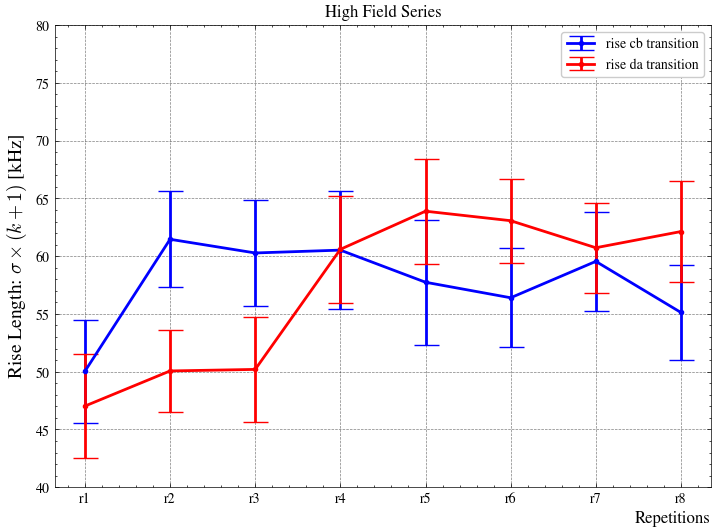
\includegraphics[width=0.75\linewidth]{figures/chapter 4/rise_s7.png} \\
    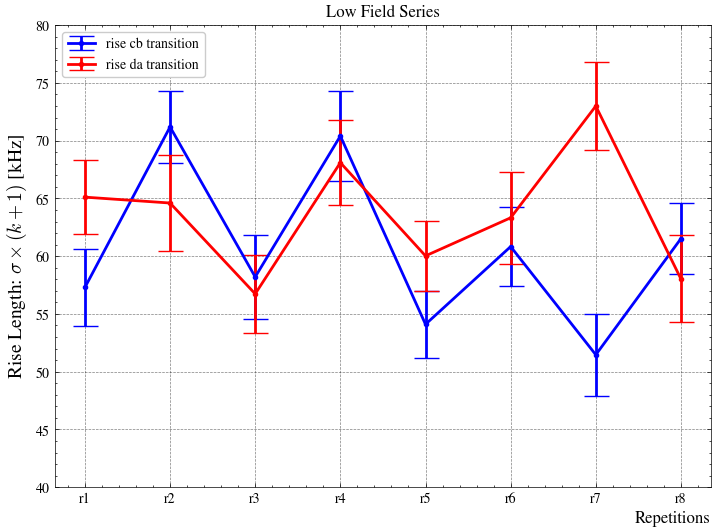
\includegraphics[width=0.75\linewidth]{figures/chapter 4/rise_s8.png}
    \caption{Length of the rising edge when letting it vary repetition by repetition (not the nominal configuration).}
    \label{fig:free_rise}
\end{figure}

\subsection{Peak frequency marker}

In this chapter, an uncertainty source was identified as the one associated with the frequency marker itself. This systematic uncertainty has been evaluated by changing the broadening of the resolution function as explained in sec \commento{aggiungere rimando}. As a cross-check, this uncertainty was estimated by repeating the measurement, but using the peak of the spectra as the frequency marker, and calculating the difference between results in the two cases. 

In fact, the peak of the spectra is likely to be more sensitive to power variations of the injected microwave in the trap, such as those that could affect \cb and \da differently. And, as explained before, such differences between \cb and \da directly constitute a systematic uncertainty.

The result of the analysis with this different method is:

\begin{itemize}
\item For low  field series: $a_{1S}/h$ = \SI{1420406.2}{\kilo\hertz}
\item For high field series: $a_{1S}/h$ = \SI{1420405.6}{\kilo\hertz}
\end{itemize}

These values give an uncertainty smaller than the one that was used for the error budget. Since this represents a worst-case scenario, this adds confidence that this contribution is under control.

\subsection{Z and Radius variable selection}

A validation has been performed by applying a $Z$ and radius selection in addition to the MVA classifier already considered. The analysis has been repeated for two complementary $Z$ cut selections, considering firstly all the annihilations above the mean of the Z distribution and secondly the ones below (see Fig.~\ref{fig:ZcutSelection}). This test was carried out to search for inconsistencies in the annihilation pattern, and the results obtained are compatible with one another, indicating no evidence of a dependence of the analysis result on the Z variable at the current resolution level.
A similar study was conducted using alternative radius cuts. Radius selections can help reveal possible contributions from residual-gas annihilations, which are expected to occur at a smaller radius than induced spin-flip annihilations: residual-gas annihilations can happen anywhere inside the trap volume, whereas spin-flip annihilations occur on the trap wall, at a larger value. Naturally, due to detector resolution, the reconstructed radius distribution is smeared between these two regimes, blurring the distinction. A summary of these studies is contained in Tab.~\ref{tab:selections}


\begin{figure}[!hbtp]
\centering
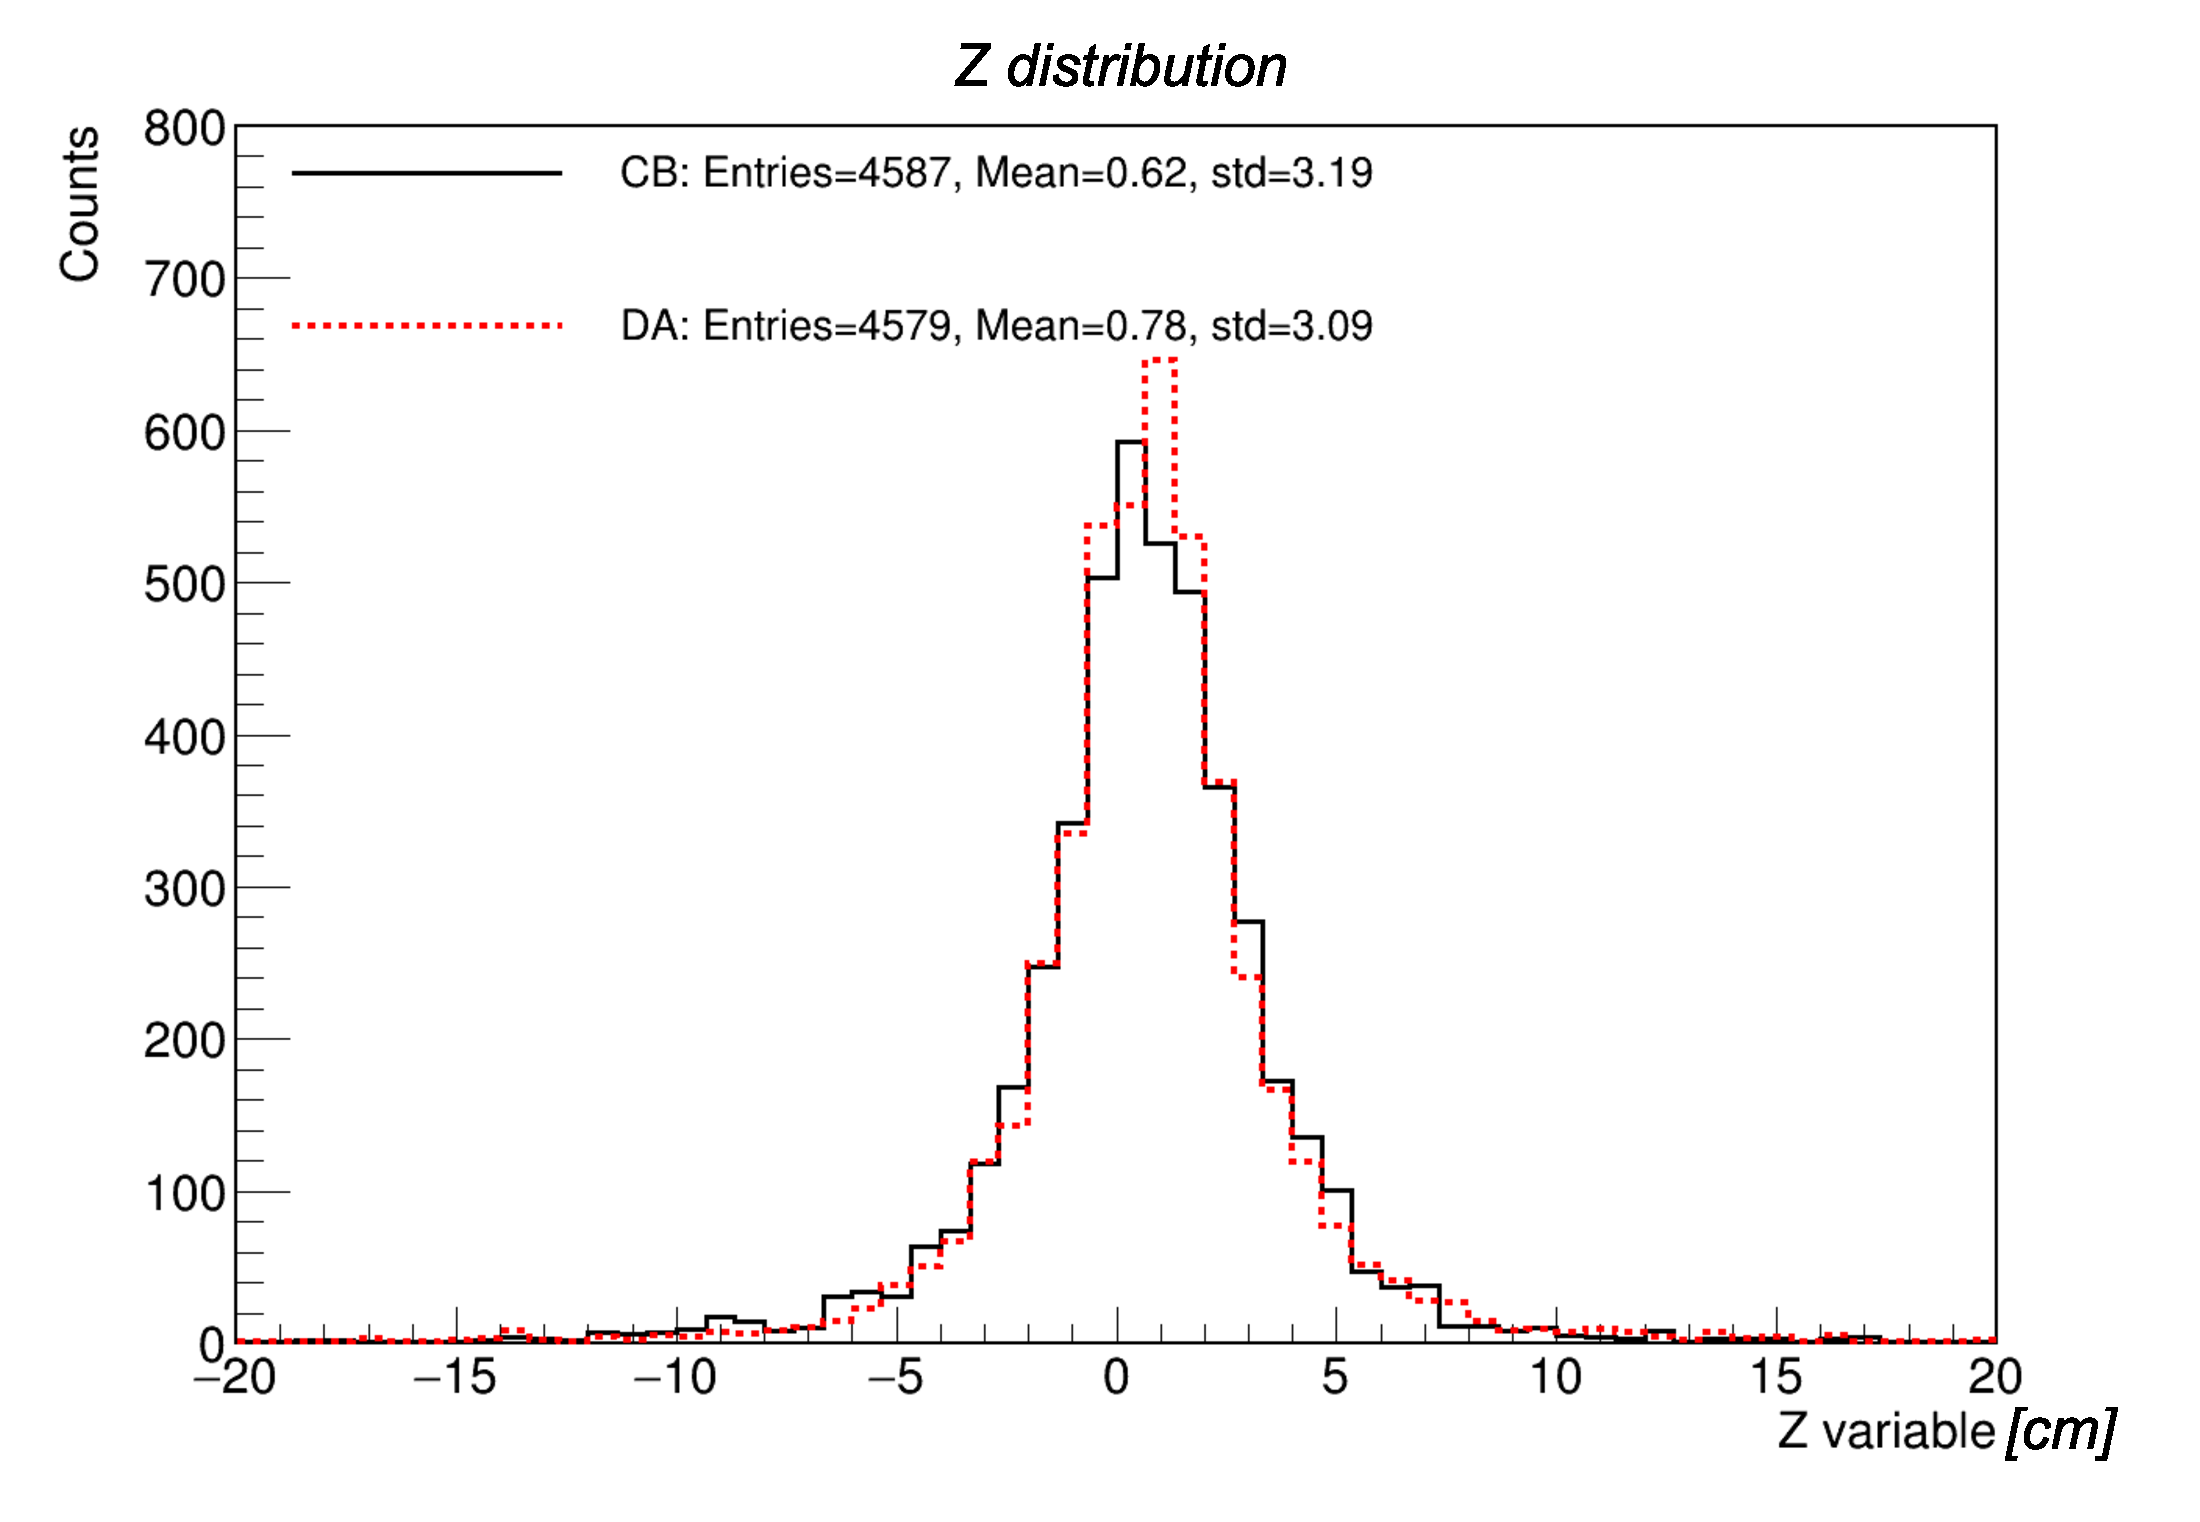
\includegraphics[width = 0.95\textwidth]{figures/chapter 4/Z_s7.pdf} \\
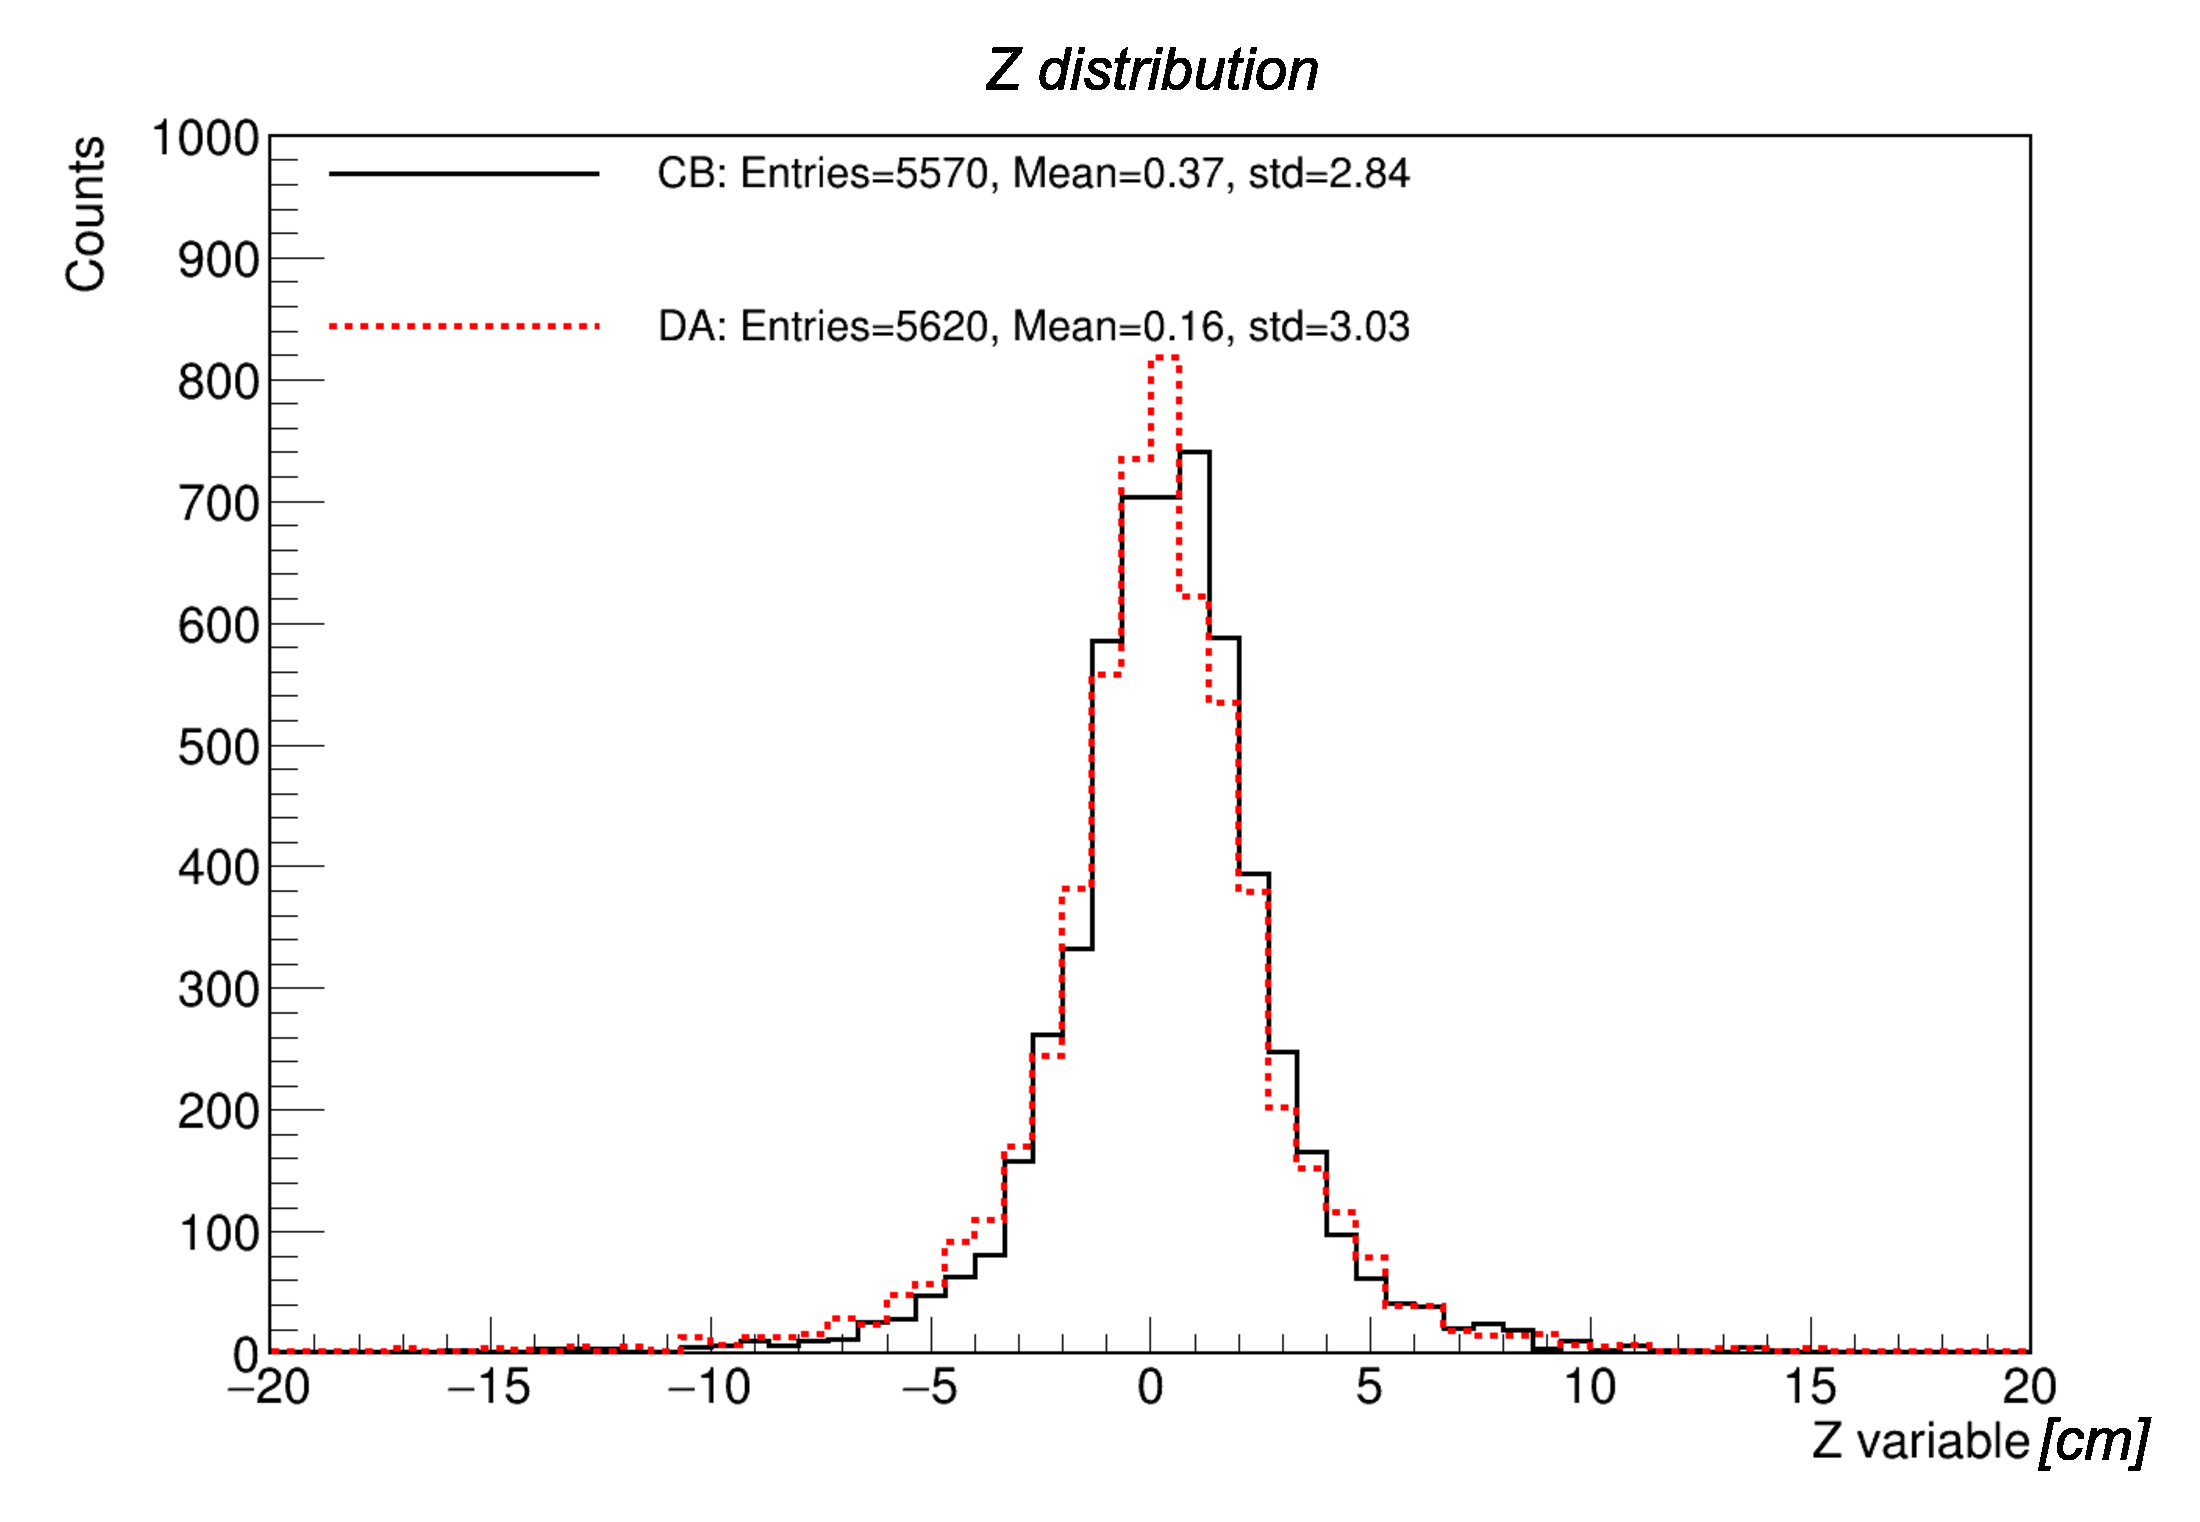
\includegraphics[width = 0.95\textwidth]{figures/chapter 4/Z_s8.pdf}
\caption{Distribution of the $Z$ variable of the annihilation vertices for the high field series (top plot) and low field series (bottom plot). Each plot shows two distributions: the $Z$ distribution for annihilations during the \cb measurement (black continuous line) and during the \da measurement (red dotted lines). The distribution contains all the accumulated events of the eight repetitions.}
\label{fig:ZcutSelection}
\end{figure}



\begin{table}[!h]
\centering							
\begin{tabular}{l||r|l||r|l}					
\hline
\hline								
\textbf{Configuration} & \multicolumn{2}{c||}{\textbf{\SI{1.07}{\tesla} dataset}} & \multicolumn{2}{c}{\textbf{\SI{1.03}{\tesla} dataset}} \\
 & $	\mu	\pm	\sigma \;({\rm kHz})$ & $	\bf{\Delta}	\;({\rm kHz})$ & $	\mu	\pm	\sigma	\;({\rm kHz}) $ & $	\bf{\Delta}	\;({\rm kHz})$ \\
\hline
\hline
{\bf \textcolor{blue}{Nominal}}	& {\textcolor{blue}{10.84 $\pm$ 1.7}} &$- $& {\textcolor{blue}{8.98 $\pm$ 1.5 }}& $ - $ \\
\hline
\hline
$1.5< r< 4\,{\rm cm}$ & $ 10.09 \pm 1.9 $ & $ -0.8 $& $ 6.95 \pm 1.7 $ & $ -2.03  $ \\
$ |z|<5\,{\rm cm}$    & $9.65 \pm 1.7$ & $-1.2 $& $9.92 \pm 1.5$ & $ +1.0 $ \\
\hline
\hline
 $Z_{cb} > 0.62 $ \& $Z_{da} > 0.78$ & $ 12.3 \pm 2.4 $ & $ 1.4$ & N/A & N/A\\
 $Z_{cb} < 0.62 $ \& $Z_{da} < 0.78$ & $ 9.9 \pm 2.4  $ & $-0.9$ & N/A & N/A\\
\hline
 $Z_{cb} >$ 0.37  \& $Z_{da} > 0.16$ & N/A & N/A & $8.00  \pm 2.1$ & $ -1.0 $ \\
 $Z_{cb} <$ 0.37  \& $Z_{da} < 0.16$ & N/A & N/A & $10.32 \pm 2.0$ & $ +1.3$\\

\hline
\hline
\end{tabular}
\caption{Comparison of the results with geometrical selections. The results reported in the table are blinded. The Nominal value corresponds to the blind result of the analysis. The systematic shift is the result of the difference between the values reported in the nominal row and the other values reported in the following rows.}
\label{tab:selections}
\end{table}

